\documentclass[]{book}
\usepackage{lmodern}
\usepackage{amssymb,amsmath}
\usepackage{ifxetex,ifluatex}
\usepackage{fixltx2e} % provides \textsubscript
\ifnum 0\ifxetex 1\fi\ifluatex 1\fi=0 % if pdftex
  \usepackage[T1]{fontenc}
  \usepackage[utf8]{inputenc}
\else % if luatex or xelatex
  \ifxetex
    \usepackage{mathspec}
  \else
    \usepackage{fontspec}
  \fi
  \defaultfontfeatures{Ligatures=TeX,Scale=MatchLowercase}
\fi
% use upquote if available, for straight quotes in verbatim environments
\IfFileExists{upquote.sty}{\usepackage{upquote}}{}
% use microtype if available
\IfFileExists{microtype.sty}{%
\usepackage{microtype}
\UseMicrotypeSet[protrusion]{basicmath} % disable protrusion for tt fonts
}{}
\usepackage[margin=1in]{geometry}
\usepackage{hyperref}
\hypersetup{unicode=true,
            pdftitle={Introduction to R Programming},
            pdfauthor={David Beskow},
            pdfborder={0 0 0},
            breaklinks=true}
\urlstyle{same}  % don't use monospace font for urls
\usepackage{natbib}
\bibliographystyle{apalike}
\usepackage{color}
\usepackage{fancyvrb}
\newcommand{\VerbBar}{|}
\newcommand{\VERB}{\Verb[commandchars=\\\{\}]}
\DefineVerbatimEnvironment{Highlighting}{Verbatim}{commandchars=\\\{\}}
% Add ',fontsize=\small' for more characters per line
\usepackage{framed}
\definecolor{shadecolor}{RGB}{248,248,248}
\newenvironment{Shaded}{\begin{snugshade}}{\end{snugshade}}
\newcommand{\KeywordTok}[1]{\textcolor[rgb]{0.13,0.29,0.53}{\textbf{{#1}}}}
\newcommand{\DataTypeTok}[1]{\textcolor[rgb]{0.13,0.29,0.53}{{#1}}}
\newcommand{\DecValTok}[1]{\textcolor[rgb]{0.00,0.00,0.81}{{#1}}}
\newcommand{\BaseNTok}[1]{\textcolor[rgb]{0.00,0.00,0.81}{{#1}}}
\newcommand{\FloatTok}[1]{\textcolor[rgb]{0.00,0.00,0.81}{{#1}}}
\newcommand{\ConstantTok}[1]{\textcolor[rgb]{0.00,0.00,0.00}{{#1}}}
\newcommand{\CharTok}[1]{\textcolor[rgb]{0.31,0.60,0.02}{{#1}}}
\newcommand{\SpecialCharTok}[1]{\textcolor[rgb]{0.00,0.00,0.00}{{#1}}}
\newcommand{\StringTok}[1]{\textcolor[rgb]{0.31,0.60,0.02}{{#1}}}
\newcommand{\VerbatimStringTok}[1]{\textcolor[rgb]{0.31,0.60,0.02}{{#1}}}
\newcommand{\SpecialStringTok}[1]{\textcolor[rgb]{0.31,0.60,0.02}{{#1}}}
\newcommand{\ImportTok}[1]{{#1}}
\newcommand{\CommentTok}[1]{\textcolor[rgb]{0.56,0.35,0.01}{\textit{{#1}}}}
\newcommand{\DocumentationTok}[1]{\textcolor[rgb]{0.56,0.35,0.01}{\textbf{\textit{{#1}}}}}
\newcommand{\AnnotationTok}[1]{\textcolor[rgb]{0.56,0.35,0.01}{\textbf{\textit{{#1}}}}}
\newcommand{\CommentVarTok}[1]{\textcolor[rgb]{0.56,0.35,0.01}{\textbf{\textit{{#1}}}}}
\newcommand{\OtherTok}[1]{\textcolor[rgb]{0.56,0.35,0.01}{{#1}}}
\newcommand{\FunctionTok}[1]{\textcolor[rgb]{0.00,0.00,0.00}{{#1}}}
\newcommand{\VariableTok}[1]{\textcolor[rgb]{0.00,0.00,0.00}{{#1}}}
\newcommand{\ControlFlowTok}[1]{\textcolor[rgb]{0.13,0.29,0.53}{\textbf{{#1}}}}
\newcommand{\OperatorTok}[1]{\textcolor[rgb]{0.81,0.36,0.00}{\textbf{{#1}}}}
\newcommand{\BuiltInTok}[1]{{#1}}
\newcommand{\ExtensionTok}[1]{{#1}}
\newcommand{\PreprocessorTok}[1]{\textcolor[rgb]{0.56,0.35,0.01}{\textit{{#1}}}}
\newcommand{\AttributeTok}[1]{\textcolor[rgb]{0.77,0.63,0.00}{{#1}}}
\newcommand{\RegionMarkerTok}[1]{{#1}}
\newcommand{\InformationTok}[1]{\textcolor[rgb]{0.56,0.35,0.01}{\textbf{\textit{{#1}}}}}
\newcommand{\WarningTok}[1]{\textcolor[rgb]{0.56,0.35,0.01}{\textbf{\textit{{#1}}}}}
\newcommand{\AlertTok}[1]{\textcolor[rgb]{0.94,0.16,0.16}{{#1}}}
\newcommand{\ErrorTok}[1]{\textcolor[rgb]{0.64,0.00,0.00}{\textbf{{#1}}}}
\newcommand{\NormalTok}[1]{{#1}}
\usepackage{longtable,booktabs}
\usepackage{graphicx,grffile}
\makeatletter
\def\maxwidth{\ifdim\Gin@nat@width>\linewidth\linewidth\else\Gin@nat@width\fi}
\def\maxheight{\ifdim\Gin@nat@height>\textheight\textheight\else\Gin@nat@height\fi}
\makeatother
% Scale images if necessary, so that they will not overflow the page
% margins by default, and it is still possible to overwrite the defaults
% using explicit options in \includegraphics[width, height, ...]{}
\setkeys{Gin}{width=\maxwidth,height=\maxheight,keepaspectratio}
\IfFileExists{parskip.sty}{%
\usepackage{parskip}
}{% else
\setlength{\parindent}{0pt}
\setlength{\parskip}{6pt plus 2pt minus 1pt}
}
\setlength{\emergencystretch}{3em}  % prevent overfull lines
\providecommand{\tightlist}{%
  \setlength{\itemsep}{0pt}\setlength{\parskip}{0pt}}
\setcounter{secnumdepth}{5}
% Redefines (sub)paragraphs to behave more like sections
\ifx\paragraph\undefined\else
\let\oldparagraph\paragraph
\renewcommand{\paragraph}[1]{\oldparagraph{#1}\mbox{}}
\fi
\ifx\subparagraph\undefined\else
\let\oldsubparagraph\subparagraph
\renewcommand{\subparagraph}[1]{\oldsubparagraph{#1}\mbox{}}
\fi

%%% Use protect on footnotes to avoid problems with footnotes in titles
\let\rmarkdownfootnote\footnote%
\def\footnote{\protect\rmarkdownfootnote}

%%% Change title format to be more compact
\usepackage{titling}

% Create subtitle command for use in maketitle
\newcommand{\subtitle}[1]{
  \posttitle{
    \begin{center}\large#1\end{center}
    }
}

\setlength{\droptitle}{-2em}
  \title{Introduction to R Programming}
  \pretitle{\vspace{\droptitle}\centering\huge}
  \posttitle{\par}
  \author{David Beskow}
  \preauthor{\centering\large\emph}
  \postauthor{\par}
  \predate{\centering\large\emph}
  \postdate{\par}
  \date{2017-04-10}

\usepackage{booktabs}
\usepackage{amsthm}
\makeatletter
\def\thm@space@setup{%
  \thm@preskip=8pt plus 2pt minus 4pt
  \thm@postskip=\thm@preskip
}
\makeatother

\begin{document}
\maketitle

{
\setcounter{tocdepth}{1}
\tableofcontents
}
These five lessons are designed to provide a person with the fundamental
understanding of the R Programming language. It will cover data
structures, data manipulation, as well as basic data visualization. The
recommended learning approach is to install R and RStudio on a computer
or cloud node, and follow along with the provided material and videos.

\chapter{Basic Data Structures}\label{basic-data-structures}

\section{The R Programming Language}\label{the-r-programming-language}

R is an extremely powerful statistical scripting language. It is
open-source and used broadly across academia, research organizations,
and businesses. It is often the tool of choice for data scientists, data
analysts, quantitative financial analysts, and a myriad of other
professions. It is used for research at the vast majority of graduate
schools. It is currently used by companies like Facebook, Google, the NY
Times and Wallstreet financial organizations. Microsoft has invested
heavily in integrating R into its desktop and cloud data science tools.
Google has written the R Style Guide that is widely used. Facebook data
scientists use R to analyze and understand the vast Facebook social
network.

\begin{figure}[htbp]
\centering
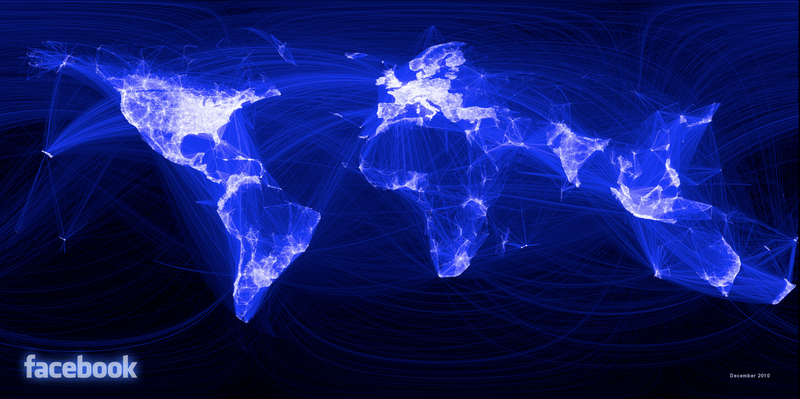
\includegraphics{facebook.png}
\caption{Figure 1: Facebook created this image with R to show how
Facebook connects the world}
\end{figure}

\subsection{R or Python?}\label{r-or-python}

The world is quickly moving toward leveraging open source data science
tools rather than proprietary software. Over the last 5 years R and
Python have risen as the two primary open source tools used by data
professionals. While there is significant overlap in the capabilities of
both languages, in general the R Programming language is better at data
analysis and visualization, and Python is better at data acquisition and
producing code for production environments. We decided to teach R in
this class since it generally has better visualizations, allowing our
analysts to tell the data narrative. Additionally, R is generally more
accessible across the Department of Defense.

\begin{figure}[htbp]
\centering
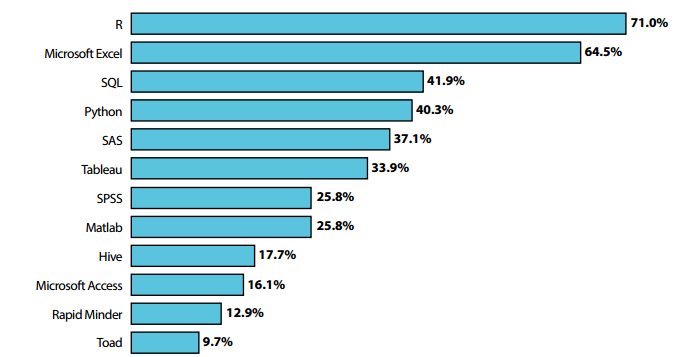
\includegraphics{whyR2.PNG}
\caption{Figure 2: LAVASTORM 2014 Survey of Industry: Primary tools used
by data scientists}
\end{figure}

R is open-source and is freely available to download. You can use base R
as-is to write and run R scripts. That being said, RStudio has provided
a very useful Integrated Development Environment (IDE) or ``front-end''
for R that is generally easier to use (R is still the ``engine''; you
can't run RStudio without R). We will primarily use RStudio in this
course.

Note that you can also run R from a server in the ``cloud''. The Army
Data Science Center of Education (DSCOE) provides several tutorials that
explain how to do this.

\begin{center}\rule{0.5\linewidth}{\linethickness}\end{center}

\section{Installation}\label{installation}

\begin{enumerate}
\def\labelenumi{\arabic{enumi}.}
\tightlist
\item
  Install Base R by going to
  \url{http://cran.r-project.org/bin/windows/base/}
\item
  Install RStudio by going to
  \url{http://www.rstudio.com/products/rstudio/download/}
\end{enumerate}

\section{R Environment and Workspace}\label{r-environment-and-workspace}

Introductory Video:

R is always pointing to a specific directory (or folder) on your
computer. This is called your \emph{working directory}. R will always
directly read files and write files to this directory. You can see your
working directory by typing

\begin{Shaded}
\begin{Highlighting}[]
\KeywordTok{getwd}\NormalTok{()}
\end{Highlighting}
\end{Shaded}

\begin{verbatim}
## [1] "/home/dmbeskow/Dropbox/bookdown-demo-master"
\end{verbatim}

If you want to change where your working directory is, you can do this
three ways. If you are using RStudio, you can go to \emph{Session
-\textgreater{} Set Working Directory}. You can also use the
\emph{Files} tab to navigate to your desired working directory, and then
click on \emph{More -\textgreater{} Set as Working Directory}. If you
want to change your \emph{working directory} using a command (especially
if you're using base R), then you can type

\begin{Shaded}
\begin{Highlighting}[]
\KeywordTok{setwd}\NormalTok{(}\StringTok{"C:/Users/beskow/Documents"}\NormalTok{)  ###Make sure you use Forward Slashes in Windows}
\end{Highlighting}
\end{Shaded}

If you want to see the names of files in your working directory without
opening Windows Explorer, you can use the command

\begin{Shaded}
\begin{Highlighting}[]
\KeywordTok{dir}\NormalTok{()}
\end{Highlighting}
\end{Shaded}

\begin{verbatim}
##  [1] "01-fundamentals.Rmd"  "02-munging.Rmd"       "03-visualization.Rmd"
##  [4] "04-control.Rmd"       "05-dates.Rmd"         "06-references.Rmd"   
##  [7] "_book"                "book.bib"             "bookdown-demo_files" 
## [10] "bookdown-demo.Rmd"    "bookdown-demo.Rproj"  "_bookdown_files"     
## [13] "_bookdown.yml"        "_build.sh"            "dataframe.PNG"       
## [16] "dataWrangling.jpg"    "_deploy.sh"           "DESCRIPTION"         
## [19] "dplyr.png"            "environment.PNG"      "facebook.png"        
## [22] "filterColumn.PNG"     "filterRow.PNG"        "index.Rmd"           
## [25] "KoreanConflict.csv"   "LICENSE"              "list.PNG"            
## [28] "matrix.PNG"           "_output.yml"          "packages.bib"        
## [31] "preamble.tex"         "rating2.csv"          "README.md"           
## [34] "screen1.png"          "style.css"            "summer.csv"          
## [37] "tidyr.png"            "toc.css"              "vector.PNG"          
## [40] "whyR2.PNG"            "whyR.PNG"
\end{verbatim}

Note that this gives the names of the files in your working directory,
which saves you the time of opening up Windows Explorer to remind
yourself what you named your data file.

\section{Types and Shape of Data}\label{types-and-shape-of-data}

Before we get into data, I first want to show you that your command line
can operate like a calculator

\begin{Shaded}
\begin{Highlighting}[]
\DecValTok{5} \NormalTok{+}\StringTok{ }\DecValTok{4} \NormalTok{+}\StringTok{ }\DecValTok{7} \NormalTok{*}\StringTok{ }\DecValTok{7}
\end{Highlighting}
\end{Shaded}

\begin{verbatim}
## [1] 58
\end{verbatim}

or

\begin{Shaded}
\begin{Highlighting}[]
\NormalTok{pi *}\StringTok{ }\FloatTok{7.2}\NormalTok{^}\DecValTok{2}
\end{Highlighting}
\end{Shaded}

\begin{verbatim}
## [1] 162.8602
\end{verbatim}

Note that in both of these examples, the answer is printed to the
screen, but not stored in memory. In other words, I cannot access that
answer without redoing the calculation. If I want to store it in memory,
then I assign the answer to a name. We use the symbol \textless{}- to
mean ``assign''. In other words, the result of the computation on the
right of the symbol is assigned to the name on the left of the symbol.
For example:

\begin{Shaded}
\begin{Highlighting}[]
\NormalTok{x <-}\StringTok{ }\DecValTok{4}\NormalTok{*}\DecValTok{4}
\end{Highlighting}
\end{Shaded}

I have now assigned the result of my computation to the name \emph{x}.
If I want to see this value of \emph{x} in the future, I can just type
it in the console.

\begin{Shaded}
\begin{Highlighting}[]
\NormalTok{x}
\end{Highlighting}
\end{Shaded}

\begin{verbatim}
## [1] 16
\end{verbatim}

Note that in \emph{RStudio} you can also see your variable in the
\emph{Environment} window.

I can also use it in future computations:

\begin{Shaded}
\begin{Highlighting}[]
\NormalTok{y<-x/}\DecValTok{2}
\end{Highlighting}
\end{Shaded}

\emph{x} is now stored in your \emph{Global Environment}. Think of this
as your ``workbench'' that contains all of the data and values that you
are working on. In RStudio, you can usually see what is in your
\emph{Global Environment} in the top right part of the RStudio window.

\begin{figure}[htbp]
\centering
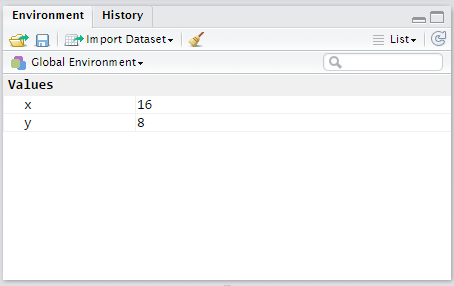
\includegraphics{environment.PNG}
\caption{Figure 3: The ``Environment'' window shows the name and type of
data held in memory}
\end{figure}

If you're using base R, you can list the variables that are in your
\emph{Global Environment} by typing

\begin{Shaded}
\begin{Highlighting}[]
\KeywordTok{ls}\NormalTok{()}
\end{Highlighting}
\end{Shaded}

\begin{verbatim}
## [1] "x" "y"
\end{verbatim}

When you close either RStudio or base R, it will ask you if you want to
save your \emph{work space}. It is essentially asking you if you want to
save what is on your workbench. If you choose ``yes'', then it will save
an *.RData file of everything that is in your workspace in your working
directory. If you restart R from this working directory, it will load
all of these items into your workspace. Generally it is not a good idea
to save your workspace as long as you have all of the code it would take
to quickly recreate all of the items in your workspace. However, if you
have some code that takes along time to run, then it is best to save
these items in a workspace so that you don't have to wait hours/days a
second time to recreate them. For example, I created some R code to
``clean'' operational combat data. It took approximately 11 days to
clean the data. In this case, I would want to save my results so I don't
have to wait 11 days again for this to run. In general, however, R takes
seconds to run, and it is best to not save your workspace as long as you
have clean and easy to run code.

\section{Data Types}\label{data-types}

Now that we have R and RStudio installed, let's look at different
classes of data. The basic building blocks are \emph{integer},
\emph{numeric}, \emph{character}, \emph{date}, \emph{boolean} (logical)
or \emph{factor} classes of data. The first four should be self
explanatory, and examples of all four are below:

\begin{Shaded}
\begin{Highlighting}[]
\NormalTok{x<-}\DecValTok{4}                   \CommentTok{#integer}
\NormalTok{x<-}\FloatTok{4.56}                \CommentTok{#numeric}
\NormalTok{x<-}\OtherTok{TRUE}                \CommentTok{#boolean}
\NormalTok{x<-}\StringTok{"Rangers Lead the Way!"}  \CommentTok{#character}
\end{Highlighting}
\end{Shaded}

Use the class command to find out what type of data you have. Note that
because we were using \emph{x} for all three, that we were writing over
the value of x. At the end of running these four lines of code, \emph{x}
would equal the last line of code: the character string ``Rangers Lead
the Way!''

\begin{Shaded}
\begin{Highlighting}[]
\KeywordTok{class}\NormalTok{(x)}
\end{Highlighting}
\end{Shaded}

\begin{verbatim}
## [1] "character"
\end{verbatim}

R does not automatically recognize \emph{date} data. When you read
\emph{date} data into R, it is initially converted to \emph{character}
data. If you want R to recognize it as a \emph{date}, you need to
explicity change it (we will go over this in more detail later):

\begin{Shaded}
\begin{Highlighting}[]
\NormalTok{x<-}\StringTok{"2014-01-01"}
\NormalTok{x<-}\KeywordTok{as.Date}\NormalTok{(x)}
\KeywordTok{class}\NormalTok{(x)}
\end{Highlighting}
\end{Shaded}

\begin{verbatim}
## [1] "Date"
\end{verbatim}

There is also a type of data called \emph{factor} data. This is
categorical data (often a character string) that has a numeric value
tied to it for certain types of models. Character data is often coerced
to the \emph{factor} class when you have nominal data (for example, a
\emph{gender} field that contained the strings ``male'' and ``female'').
If I change this into a factor, it will still be represented as ``male''
and ``female'', but it will also be represented numerically (as a 1 and
2). You need to be very careful when using factors, since many of the
functions in R can't handle factor data. You can see the use of factor
data below:

\begin{Shaded}
\begin{Highlighting}[]
\NormalTok{y<-}\KeywordTok{c}\NormalTok{(}\StringTok{"male"}\NormalTok{,}\StringTok{"male"}\NormalTok{,}\StringTok{"female"}\NormalTok{,}\StringTok{"male"}\NormalTok{,}\StringTok{"female"}\NormalTok{)}
\end{Highlighting}
\end{Shaded}

This is character data. If I tried to plot y right now, R would show an
error, since you can't print \emph{character} data. Lets convert this to
a factor now:

\begin{Shaded}
\begin{Highlighting}[]
\NormalTok{y<-}\KeywordTok{as.factor}\NormalTok{(y)}
\NormalTok{y}
\end{Highlighting}
\end{Shaded}

\begin{verbatim}
## [1] male   male   female male   female
## Levels: female male
\end{verbatim}

Now watch when I try to plot this:

\begin{Shaded}
\begin{Highlighting}[]
\KeywordTok{plot}\NormalTok{(y)}
\end{Highlighting}
\end{Shaded}

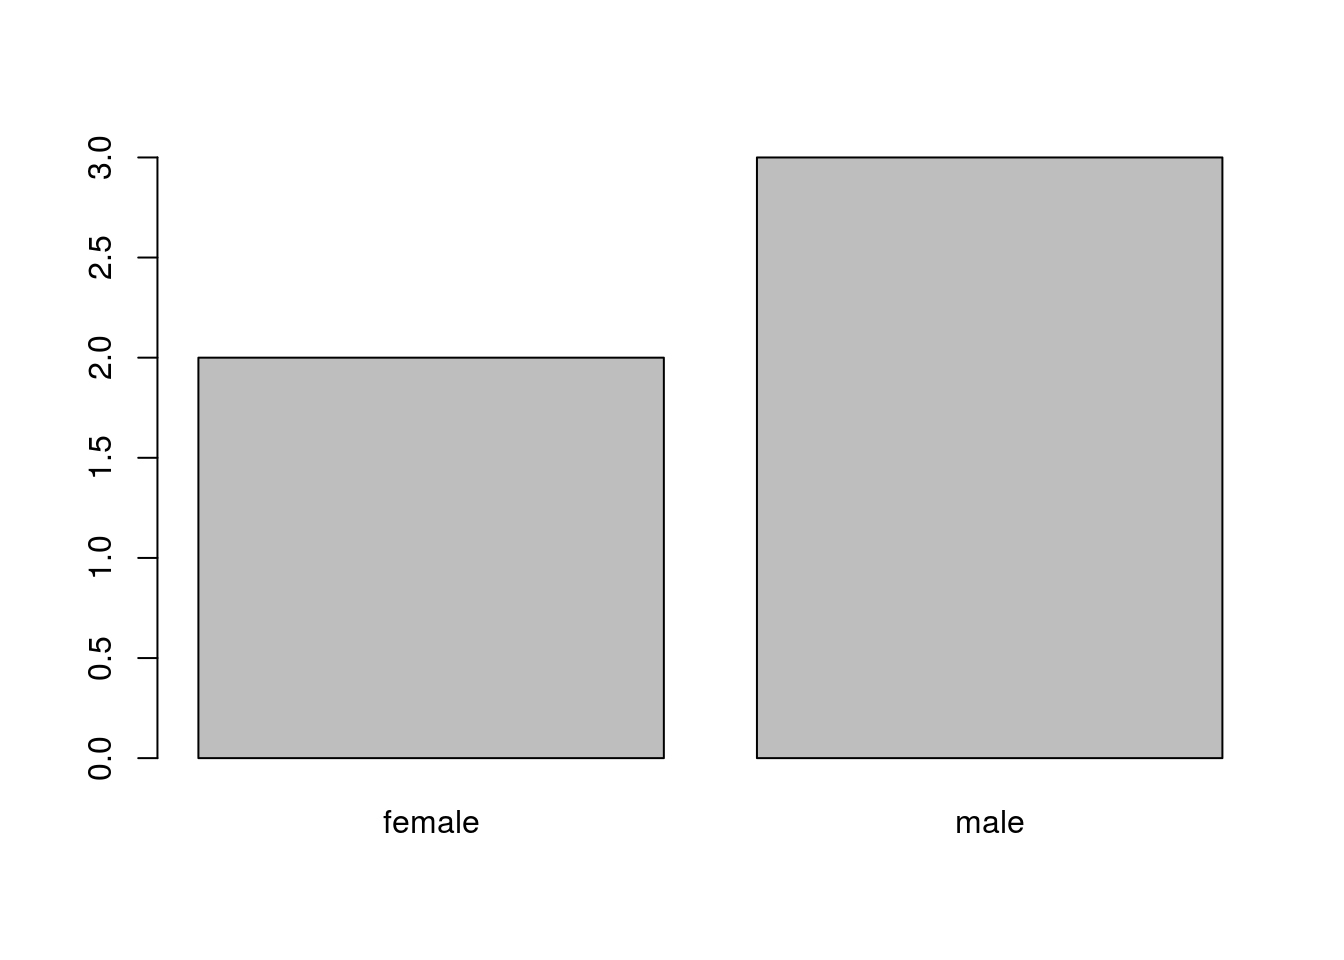
\includegraphics{bookdown-demo_files/figure-latex/unnamed-chunk-16-1.pdf}

It plots a barchart because R recognizes this as a factor and has a
numeric value associated with both of the ``levels'' in the factor

\section{Data Structures}\label{data-structures}

The data that we showed above is trivial (and very small) data. To work
with data, we'd prefer to have it organized into a usable data
structure. In this section we will introduce you to the four primary
data structures that we will use:

\begin{longtable}[]{@{}ll@{}}
\toprule
\begin{minipage}[b]{0.18\columnwidth}\raggedright\strut
Data Structure\strut
\end{minipage} & \begin{minipage}[b]{0.24\columnwidth}\raggedright\strut
Definition\strut
\end{minipage}\tabularnewline
\midrule
\endhead
\begin{minipage}[t]{0.18\columnwidth}\raggedright\strut
Vector\strut
\end{minipage} & \begin{minipage}[t]{0.24\columnwidth}\raggedright\strut
Data in one dimension\strut
\end{minipage}\tabularnewline
\begin{minipage}[t]{0.18\columnwidth}\raggedright\strut
Data Frame\strut
\end{minipage} & \begin{minipage}[t]{0.24\columnwidth}\raggedright\strut
Two dimensional data (most commonly used data structure)\strut
\end{minipage}\tabularnewline
\begin{minipage}[t]{0.18\columnwidth}\raggedright\strut
List\strut
\end{minipage} & \begin{minipage}[t]{0.24\columnwidth}\raggedright\strut
A one dimensional data structure that can contain any class of data
(objects could be other data structures)\strut
\end{minipage}\tabularnewline
\begin{minipage}[t]{0.18\columnwidth}\raggedright\strut
Matrix\strut
\end{minipage} & \begin{minipage}[t]{0.24\columnwidth}\raggedright\strut
Multi-dimensional data of the same class\strut
\end{minipage}\tabularnewline
\bottomrule
\end{longtable}

There are also different dimensions of data. So far we've been using
\emph{scalars}, in which our variable x is a single value. Data can have
1, 2, or many dimensions, however.

\subsection{Vector Data Structure}\label{vector-data-structure}

One dimensional data that is of the same class is often organized into a
\emph{vector}. All objects in a vector must be of the same class (or
will be coerced to the same class). A picture of a vector is given below

\begin{figure}[htbp]
\centering
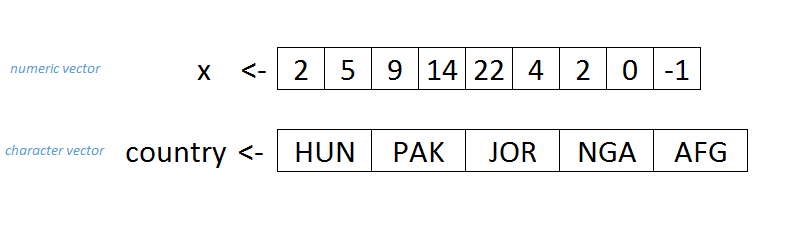
\includegraphics{vector.PNG}
\caption{Figure 4: Understanding Vector Data in R}
\end{figure}

An example of a vector in R is given below:

\begin{Shaded}
\begin{Highlighting}[]
\NormalTok{x<-}\KeywordTok{c}\NormalTok{(}\DecValTok{1}\NormalTok{,}\DecValTok{6}\NormalTok{,}\DecValTok{3}\NormalTok{,}\DecValTok{9}\NormalTok{,}\DecValTok{8}\NormalTok{,}\DecValTok{2}\NormalTok{)    ## "c" means combine the values into a vector}
\end{Highlighting}
\end{Shaded}

If you need to create a vector of sequential integers, you can use a
colon:

\begin{Shaded}
\begin{Highlighting}[]
\NormalTok{x<-}\KeywordTok{c}\NormalTok{(}\DecValTok{1}\NormalTok{:}\DecValTok{10}\NormalTok{)}
\NormalTok{x}
\end{Highlighting}
\end{Shaded}

\begin{verbatim}
##  [1]  1  2  3  4  5  6  7  8  9 10
\end{verbatim}

If you need to create a vector of the same number, you can use the
repeat command:

\begin{Shaded}
\begin{Highlighting}[]
\KeywordTok{rep}\NormalTok{(}\DecValTok{1}\NormalTok{,}\DecValTok{10}\NormalTok{)  }\CommentTok{# Repeat 1 ten times}
\end{Highlighting}
\end{Shaded}

\begin{verbatim}
##  [1] 1 1 1 1 1 1 1 1 1 1
\end{verbatim}

\subsection{Data Frame Data Structure}\label{data-frame-data-structure}

Anyone who has used Microsoft Excel is used to seeing data in the
traditional two dimensional table. The data frame structures data in
this way. A picture of a data frame is provided below:

\begin{figure}[htbp]
\centering
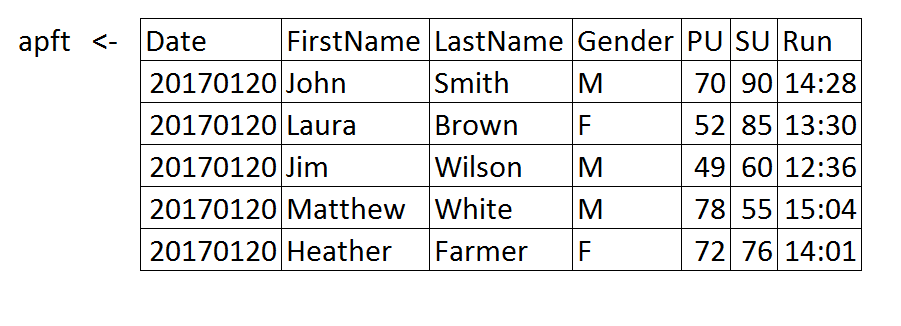
\includegraphics{dataframe.PNG}
\caption{Figure 5: Understanding Data Frame Structure in R}
\end{figure}

Each column of a data frame is a vector, and must have the same class of
data. A data frame is a list of vectors where each each vector has the
same length. A data frame is usually created when you read data from an
external file (usually a CSV file), but you can create one manually, as
seen below:

\begin{Shaded}
\begin{Highlighting}[]
\NormalTok{##Create a data frame}
\NormalTok{apft <-}\StringTok{ }\KeywordTok{data.frame}\NormalTok{(}\DataTypeTok{Name =} \KeywordTok{c}\NormalTok{(}\StringTok{"John"}\NormalTok{,}\StringTok{"Laura"}\NormalTok{,}\StringTok{"Jim"}\NormalTok{),}
                   \DataTypeTok{Gender =} \KeywordTok{c}\NormalTok{(}\StringTok{"M"}\NormalTok{,}\StringTok{"F"}\NormalTok{,}\StringTok{"M"}\NormalTok{),}
                   \DataTypeTok{PU =} \KeywordTok{c}\NormalTok{(}\DecValTok{70}\NormalTok{, }\DecValTok{52}\NormalTok{, }\DecValTok{49}\NormalTok{),}
                   \DataTypeTok{SU =} \KeywordTok{c}\NormalTok{(}\DecValTok{90}\NormalTok{, }\DecValTok{85}\NormalTok{, }\DecValTok{60}\NormalTok{),}
                   \DataTypeTok{Run =} \KeywordTok{c}\NormalTok{(}\StringTok{"14:28"}\NormalTok{,}\StringTok{"13:30"}\NormalTok{,}\StringTok{"12:36"}\NormalTok{))}

\NormalTok{##Print object}
\NormalTok{apft}
\end{Highlighting}
\end{Shaded}

\begin{verbatim}
##    Name Gender PU SU   Run
## 1  John      M 70 90 14:28
## 2 Laura      F 52 85 13:30
## 3   Jim      M 49 60 12:36
\end{verbatim}

\subsection{List Data Structure}\label{list-data-structure}

A list is a linear container for objects of any class or data structure.
Each object in list is separate and distinct.

A list is helpful in several situations. For example, there are many
time you have vectors that do not all have the same length. For example,
lets say we extracted hash-tags from Tweets at the Rio Olympics. The
number of hash-tags per tweet can range from zero to seven or eight (see
Figure 6 below). You can't store these vectors in a data frame because
they aren't the same length. A list is the appropriate object to store
these vectors in.

\begin{figure}[htbp]
\centering
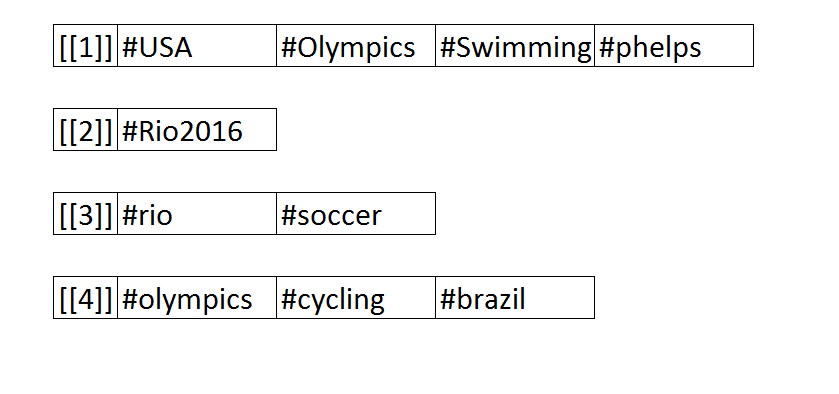
\includegraphics{list.PNG}
\caption{Figure 6: Understanding List Data Structure in R}
\end{figure}

A list is also helpful for storing different types of data in a single
object. For example, we can store a scalar, a data frame, and a vector
in a single list:

\begin{Shaded}
\begin{Highlighting}[]
\NormalTok{##Store a scalar, vector, and data frame in a list}
\NormalTok{myList <-}\StringTok{ }\KeywordTok{list}\NormalTok{(y, x, apft)}

\NormalTok{##Print object}
\NormalTok{myList}
\end{Highlighting}
\end{Shaded}

\begin{verbatim}
## [[1]]
## [1] male   male   female male   female
## Levels: female male
## 
## [[2]]
##  [1]  1  2  3  4  5  6  7  8  9 10
## 
## [[3]]
##    Name Gender PU SU   Run
## 1  John      M 70 90 14:28
## 2 Laura      F 52 85 13:30
## 3   Jim      M 49 60 12:36
\end{verbatim}

Lists also create a great container for reading multiple data files into
R and combining them into a single data frame. We will teach this
technique later.

\subsection{Matrix Data Structure}\label{matrix-data-structure}

While an important data structure in R, we will not use the matrix
structure often in this course. A matrix is a multi-dimensional array of
numeric, boolean, or integer data (NOT character, date, or factor data).

\begin{figure}[htbp]
\centering
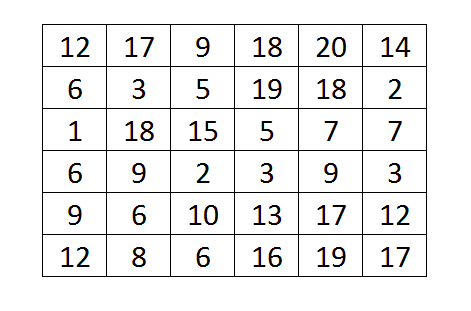
\includegraphics{matrix.PNG}
\caption{Figure 7: Understanding Matrix Data Structure in R}
\end{figure}

Below is an example of creating a matrix object in R:

\begin{Shaded}
\begin{Highlighting}[]
\NormalTok{## Example of setting row and column names}
\NormalTok{mdat <-}\StringTok{ }\KeywordTok{matrix}\NormalTok{(}\KeywordTok{c}\NormalTok{(}\DecValTok{1}\NormalTok{,}\DecValTok{2}\NormalTok{,}\DecValTok{3}\NormalTok{, }\DecValTok{11}\NormalTok{,}\DecValTok{12}\NormalTok{,}\DecValTok{13}\NormalTok{), }\DataTypeTok{nrow =} \DecValTok{2}\NormalTok{, }\DataTypeTok{ncol =} \DecValTok{3}\NormalTok{, }\DataTypeTok{byrow =} \OtherTok{TRUE}\NormalTok{)}

\NormalTok{##Print object}
\NormalTok{mdat}
\end{Highlighting}
\end{Shaded}

\begin{verbatim}
##      [,1] [,2] [,3]
## [1,]    1    2    3
## [2,]   11   12   13
\end{verbatim}

As mentioned above, we will not use matrices much in OS401.

\section{Input/Output Data}\label{inputoutput-data}

Now that we have all of that done, let's learn how to read and write
data. To do this with some fun data, let's read in some data on movie
ratings. This data contains users that rated movies in 2015. Each record
(or row) represents a single user rating a single movie. Movies can have
more than one rating, and users can rate more than one movie. Make sure
you download the data at
\url{https://s3.amazonaws.com/dscoe-data/rating2.csv} and follow along
with this tutorial.

Note: if you're using a cloud environment, you can download the data by
running the following command:

\begin{Shaded}
\begin{Highlighting}[]
\KeywordTok{download.file}\NormalTok{(}\StringTok{"https://s3.amazonaws.com/dscoe-data/rating2.csv"}\NormalTok{, }\DataTypeTok{destfile =} \StringTok{"rating2.csv"}\NormalTok{)}
\end{Highlighting}
\end{Shaded}

We use the command \emph{read.csv} to read in data. We also make sure to
assign this to an object name (in this case, the object name is
\texttt{rating})

\begin{Shaded}
\begin{Highlighting}[]
\NormalTok{rating <-}\StringTok{ }\KeywordTok{read.csv}\NormalTok{(}\StringTok{"rating2.csv"}\NormalTok{, }\DataTypeTok{as.is =} \OtherTok{TRUE}\NormalTok{)}
\end{Highlighting}
\end{Shaded}

The \texttt{as.is\ =\ TRUE} parameter ensures that any character data is
formatted into a \emph{character} vector rather than a \emph{factor}
vector. As a personal preference, I always explicitly convert to the
\emph{factor} data type when necessary so that I don't have any
undesired consequences.

Now that we've read the file in, we'll explore this data object a little
bit. Below is the top commands that I use to explore a data object.

One of the most powerful commands to explore any object is the structure
command \texttt{str}. This command gives the overall size of the object
(in this case it has 283,886 rows and 7 columns), as well as the class
of each column vector and the first few observations from each column
vector.

\begin{Shaded}
\begin{Highlighting}[]
\NormalTok{##The structure command prints the structure of the data object}
\KeywordTok{str}\NormalTok{(rating)}
\end{Highlighting}
\end{Shaded}

\begin{verbatim}
## 'data.frame':    283886 obs. of  7 variables:
##  $ userId   : int  31 31 31 31 31 31 31 31 31 31 ...
##  $ movieId  : int  1 110 260 364 527 588 594 616 1196 1197 ...
##  $ rating   : num  3 5 5 3 0.5 3 2.5 4 5 3 ...
##  $ timestamp: chr  "2015-02-23 23:18:07" "2015-02-23 23:17:53" "2015-02-23 23:17:13" "2015-02-25 06:13:27" ...
##  $ year     : int  2015 2015 2015 2015 2015 2015 2015 2015 2015 2015 ...
##  $ title    : chr  "Toy Story (1995)" "Braveheart (1995)" "Star Wars: Episode IV - A New Hope (1977)" "Lion King, The (1994)" ...
##  $ genres   : chr  "Adventure|Animation|Children|Comedy|Fantasy" "Action|Drama|War" "Action|Adventure|Sci-Fi" "Adventure|Animation|Children|Drama|Musical|IMAX" ...
\end{verbatim}

Related to the \texttt{str} command is the \texttt{summary} command.
This command is especially helpful if you have numeric data in the
object and you want to view some of the basic statistics regarding this
data.

\begin{Shaded}
\begin{Highlighting}[]
\NormalTok{##The summary command prints summary statistics about an object in memory}
\KeywordTok{summary}\NormalTok{(rating)}
\end{Highlighting}
\end{Shaded}

\begin{verbatim}
##      userId          movieId           rating     timestamp        
##  Min.   :    31   Min.   :     1   Min.   :0.5   Length:283886     
##  1st Qu.: 34847   1st Qu.:  2712   1st Qu.:3.0   Class :character  
##  Median : 69852   Median :  8644   Median :3.5   Mode  :character  
##  Mean   : 69325   Mean   : 39896   Mean   :3.5                     
##  3rd Qu.:104000   3rd Qu.: 79132   3rd Qu.:4.0                     
##  Max.   :138414   Max.   :131262   Max.   :5.0                     
##       year         title              genres         
##  Min.   :2015   Length:283886      Length:283886     
##  1st Qu.:2015   Class :character   Class :character  
##  Median :2015   Mode  :character   Mode  :character  
##  Mean   :2015                                        
##  3rd Qu.:2015                                        
##  Max.   :2015
\end{verbatim}

I usually also use the command \texttt{head} to print the first 5 rows.
This gives titles of the variables (columns) as well as a feel for the
data:

\begin{Shaded}
\begin{Highlighting}[]
\NormalTok{##The head command prints the first five rows of the data set}
\KeywordTok{head}\NormalTok{(rating)}
\end{Highlighting}
\end{Shaded}

\begin{verbatim}
##   userId movieId rating           timestamp year
## 1     31       1    3.0 2015-02-23 23:18:07 2015
## 2     31     110    5.0 2015-02-23 23:17:53 2015
## 3     31     260    5.0 2015-02-23 23:17:13 2015
## 4     31     364    3.0 2015-02-25 06:13:27 2015
## 5     31     527    0.5 2015-02-23 23:19:58 2015
## 6     31     588    3.0 2015-02-25 05:41:09 2015
##                                       title
## 1                          Toy Story (1995)
## 2                         Braveheart (1995)
## 3 Star Wars: Episode IV - A New Hope (1977)
## 4                     Lion King, The (1994)
## 5                   Schindler's List (1993)
## 6                            Aladdin (1992)
##                                            genres
## 1     Adventure|Animation|Children|Comedy|Fantasy
## 2                                Action|Drama|War
## 3                         Action|Adventure|Sci-Fi
## 4 Adventure|Animation|Children|Drama|Musical|IMAX
## 5                                       Drama|War
## 6     Adventure|Animation|Children|Comedy|Musical
\end{verbatim}

If you only want to print the names of the columns, use the
\texttt{names} command:

\begin{Shaded}
\begin{Highlighting}[]
\NormalTok{##The names command just prints the column names of a data frame}
\KeywordTok{names}\NormalTok{(rating)}
\end{Highlighting}
\end{Shaded}

\begin{verbatim}
## [1] "userId"    "movieId"   "rating"    "timestamp" "year"      "title"    
## [7] "genres"
\end{verbatim}

Finally, if we only want the dimensions of the data, we can use
\texttt{dim} to get all of the dimensions, \texttt{*nrow} to access the
number of rows, and \texttt{ncol} to access the number of columns:

\begin{Shaded}
\begin{Highlighting}[]
\NormalTok{##The dim command prints the dimensions of the object}
\KeywordTok{dim}\NormalTok{(rating)}
\end{Highlighting}
\end{Shaded}

\begin{verbatim}
## [1] 283886      7
\end{verbatim}

\begin{Shaded}
\begin{Highlighting}[]
\NormalTok{##The nrow command prints the number of rows of a data frame}
\KeywordTok{nrow}\NormalTok{(rating)}
\end{Highlighting}
\end{Shaded}

\begin{verbatim}
## [1] 283886
\end{verbatim}

\begin{Shaded}
\begin{Highlighting}[]
\NormalTok{##The ncol command prints the number of columns of a data frame}
\KeywordTok{ncol}\NormalTok{(rating)}
\end{Highlighting}
\end{Shaded}

\begin{verbatim}
## [1] 7
\end{verbatim}

\section{Getting Help}\label{getting-help}

There's several ways to get help in R. The \texttt{help} function and
the \texttt{?} function can access the documentation for packages and
functions that you have loaded into R. \texttt{help.search} and the
\texttt{??} function both search within documentation for loaded
packages. Additionally, you can use the \texttt{args} function to print
out the arguments for a function.

\begin{Shaded}
\begin{Highlighting}[]
\NormalTok{##Getting help for the str function}
\KeywordTok{help}\NormalTok{(str)}

\NormalTok{##or}
\NormalTok{?str}

\NormalTok{##Searching within documentation for "subset"}
\KeywordTok{help.search}\NormalTok{(}\StringTok{'subset'}\NormalTok{)}

\NormalTok{##or}
\NormalTok{??subset}
\end{Highlighting}
\end{Shaded}

\section{Practice Problem}\label{practice-problem}

Download the Korean War Casualty Data by downloading the Comma Separated
Value (CSV) file here:

\url{https://s3.amazonaws.com/dscoe-data/KoreanConflict.csv}

If you're using a cloud environment, you can download the data by
running the following command:

\begin{Shaded}
\begin{Highlighting}[]
\KeywordTok{download.file}\NormalTok{(}\StringTok{"https://s3.amazonaws.com/dscoe-data/KoreanConflict.csv"}\NormalTok{, }\DataTypeTok{destfile =} \StringTok{"KoreanConflict.csv"}\NormalTok{)}
\end{Highlighting}
\end{Shaded}

Read this into your R environment. Explore the data given the commands
that we leaned this lessons. We will use this data in future lessons.

\chapter{Basic Data Manipulation}\label{basic-data-manipulation}

The most time intensive task in data science endeavors is pre-processing
data. Real world data is often complex and messy. Data processing
(sometimes called ``munging'' or ``data wrangling'') cleans and
manipulates data so that it is in a form that is useful for models and
visualizations. The R programming language is one of the best tools for
manipulating data. This lesson will discuss the basics of data structure
as well as ways to subset, extract and otherwise manipulate basic data.

\begin{figure}[htbp]
\centering
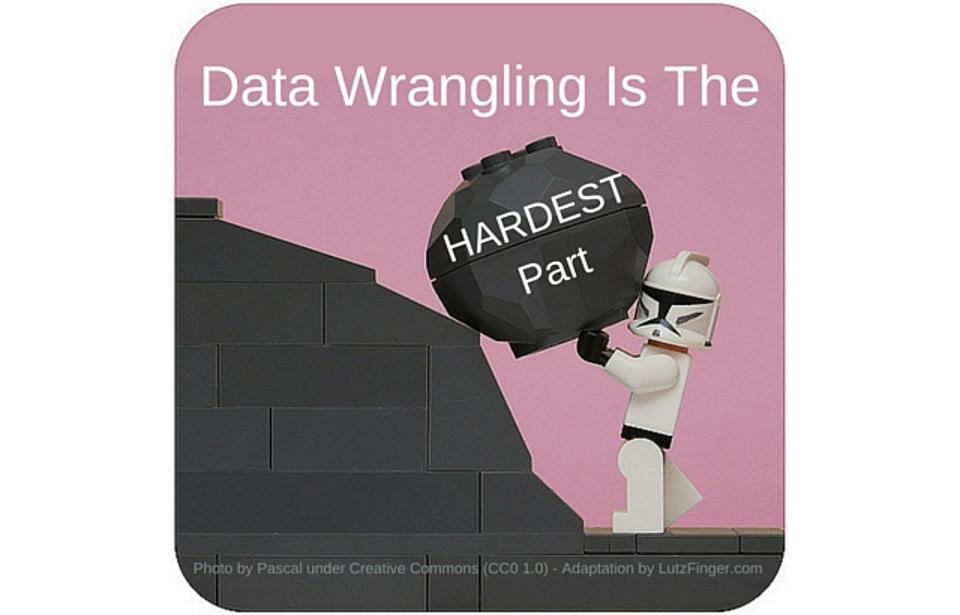
\includegraphics{dataWrangling.jpg}
\caption{Figure 1: ``Data Wrangling''" is often the most difficult part
of data science}
\end{figure}

\section{Data}\label{data}

For this lesson we will use casualty data from the Korean War. This data
is available at \href{https://www.kaggle.com/datasets}{Kaggle}. You
should have downloaded this data for the practice problem in Lesson 1.
First, let's read the data into R:

\begin{Shaded}
\begin{Highlighting}[]
\NormalTok{kor <-}\StringTok{ }\KeywordTok{read.csv}\NormalTok{(}\StringTok{"KoreanConflict.csv"}\NormalTok{, }\DataTypeTok{as.is =} \OtherTok{TRUE}\NormalTok{)}
\end{Highlighting}
\end{Shaded}

Now let's explore the data with some of the tools we learned in Lesson
1. First, let's look at the structure of the data:

\begin{Shaded}
\begin{Highlighting}[]
\KeywordTok{str}\NormalTok{(kor)  ## Print the structure of the Korean Casualty Data}
\end{Highlighting}
\end{Shaded}

\begin{verbatim}
## 'data.frame':    36574 obs. of  25 variables:
##  $ SERVICE_TYPE        : chr  "V" "R" "R" "V" ...
##  $ SERVICE_CODE        : chr  "L" "K" "K" "L" ...
##  $ ENROLLMENT          : chr  "ACTIVE - GUARD/RESERVE" "ACTIVE - REGULAR" "ACTIVE - REGULAR" "ACTIVE - GUARD/RESERVE" ...
##  $ BRANCH              : chr  "AIR FORCE" "ARMY" "ARMY" "ARMY" ...
##  $ RANK                : chr  "CAPT" "PVT" "PFC" "2LT" ...
##  $ PAY_GRADE           : chr  "O03" "E02" "E03" "O01" ...
##  $ POSITION            : chr  "" "FOOD SERVICE APPRENTICE" "HEAVY WEAPONS INFANTRYMAN" "INFANTRY UNIT COMMANDER" ...
##  $ BIRTH_YEAR          : chr  "1917" "1927" "1932" "1929" ...
##  $ SEX                 : chr  "M" "M" "M" "M" ...
##  $ HOME_CITY           : chr  "NEW YORK" "UNKNOWN" "UNKNOWN" "UNKNOWN" ...
##  $ HOME_COUNTY         : chr  "NEW YORK" "OCONEE" "BIBB" "COAHOMA" ...
##  $ NATIONALITY         : chr  "US" "US" "US" "US" ...
##  $ STATE_CODE          : chr  "NY" "GA" "GA" "MS" ...
##  $ HOME_STATE          : chr  "NEW YORK" "GEORGIA" "GEORGIA" "MISSISSIPPI" ...
##  $ MARITAL_STATUS      : chr  "MARRIED" "UNKNOWN" "UNKNOWN" "UNKNOWN" ...
##  $ ETHNICITY           : chr  "WHITE" "WHITE" "WHITE" "WHITE" ...
##  $ ETHNICITY_1         : chr  "NOT SPECIFIED" "NOT SPECIFIED" "NOT SPECIFIED" "NOT SPECIFIED" ...
##  $ ETHNICITY_2         : chr  "WHITE" "WHITE" "WHITE" "WHITE" ...
##  $ DIVISION            : chr  "93 BOMB SQ 19 BOMB GP" "29 RGT CMBT TEAM" "5 RGT 1 CAV DIV" "32 INF 7 DIV" ...
##  $ INCIDENT_DATE       : chr  "19510412" "19500727" "19510316" "19530122" ...
##  $ FATALITY_YEAR       : chr  "1951" "1950" "1951" "1953" ...
##  $ FATALITY_DATE       : chr  "20010402" "19500727" "19510316" "19530122" ...
##  $ HOSTILITY_CONDITIONS: chr  "H" "H" "H" "H" ...
##  $ FATALITY            : chr  "DECLARED DEAD" "KILLED IN ACTION" "KILLED IN ACTION" "KILLED IN ACTION" ...
##  $ BURIAL_STATUS       : chr  "Y" "Y" "Y" "Y" ...
\end{verbatim}

We see that this data has 36,574 rows and 25 columns. It appears that
each row of the data represents an individual service member who died in
the Korean War. Note that every single column is a \emph{character}
vector. This includes the rows like \texttt{BIRTH\_YEAR} and
\texttt{INCIDENT\_DATE} that appear like they should be numeric (the
fact that they are character means that at least one entry in this
column has \emph{alphabetic letters} rather than \emph{numbers}).

\section{Cell level data access}\label{cell-level-data-access}

This data set contains two dimensions (rows and columns). To access
specific rows and columns in R, we use \emph{{[}row,column{]}} format.
For example, to access the data in the first row and first column of
Korea data, we would use

\begin{Shaded}
\begin{Highlighting}[]
\NormalTok{kor[}\DecValTok{1}\NormalTok{,}\DecValTok{1}\NormalTok{]  ##First row, first column}
\end{Highlighting}
\end{Shaded}

\begin{verbatim}
## [1] "V"
\end{verbatim}

If we want to access the first 5 entries from the first column, we would
use

\begin{Shaded}
\begin{Highlighting}[]
\NormalTok{kor[}\KeywordTok{c}\NormalTok{(}\DecValTok{1}\NormalTok{:}\DecValTok{5}\NormalTok{),}\DecValTok{1}\NormalTok{] ##First five entries from the first column}
\end{Highlighting}
\end{Shaded}

\begin{verbatim}
## [1] "V" "R" "R" "V" "R"
\end{verbatim}

Now if we want to access the first three rows from the 1st, 3rd, and 8th
column, we use the following format

\begin{Shaded}
\begin{Highlighting}[]
\NormalTok{kor[}\DecValTok{1}\NormalTok{:}\DecValTok{3}\NormalTok{,}\KeywordTok{c}\NormalTok{(}\DecValTok{1}\NormalTok{,}\DecValTok{3}\NormalTok{,}\DecValTok{8}\NormalTok{)]}
\end{Highlighting}
\end{Shaded}

\begin{verbatim}
##   SERVICE_TYPE             ENROLLMENT BIRTH_YEAR
## 1            V ACTIVE - GUARD/RESERVE       1917
## 2            R       ACTIVE - REGULAR       1927
## 3            R       ACTIVE - REGULAR       1932
\end{verbatim}

You can also use column names (or headers) to extract data from specific
columns. This is especially helpful if you can't remember respective
column numbers, or if you think the column order will ever change. To
extract the first three rows of data from \texttt{BRANCH},
\texttt{RANK}, and \texttt{HOME\_STATE}, we can use the code below.

\begin{Shaded}
\begin{Highlighting}[]
\NormalTok{kor[}\DecValTok{1}\NormalTok{:}\DecValTok{3}\NormalTok{,}\KeywordTok{c}\NormalTok{(}\StringTok{"RANK"}\NormalTok{,}\StringTok{"BRANCH"}\NormalTok{,}\StringTok{"HOME_STATE"}\NormalTok{)]}
\end{Highlighting}
\end{Shaded}

\begin{verbatim}
##   RANK    BRANCH HOME_STATE
## 1 CAPT AIR FORCE   NEW YORK
## 2  PVT      ARMY    GEORGIA
## 3  PFC      ARMY    GEORGIA
\end{verbatim}

Remember that each column represents a vector. In addition to the method
we just showed, you can access data from each column vector with the
following script:

\begin{Shaded}
\begin{Highlighting}[]
\NormalTok{kor$RANK[}\DecValTok{1}\NormalTok{:}\DecValTok{5}\NormalTok{]  ##Prints first five entries in RANK vector}
\end{Highlighting}
\end{Shaded}

\begin{verbatim}
## [1] "CAPT" "PVT"  "PFC"  "2LT"  "CPL"
\end{verbatim}

The script above essentially says select the RANK column from the
\texttt{kor} data frame, and then print to the screen the first five
entries of this column.

\section{\texorpdfstring{\texttt{Table} Command (and an example of data
``cleaning'')}{Table Command (and an example of data cleaning)}}\label{table-command-and-an-example-of-data-cleaning}

Let's explore the data a bit more. The \texttt{table} command provides a
great way to see all of the possible entries in categorical data. The
table command has similar functionality to \emph{Pivot Tables} in Excel,
but is much easier to use. To illustrate this command, we will table the
\texttt{BIRTH\_YEAR}

\begin{Shaded}
\begin{Highlighting}[]
\KeywordTok{table}\NormalTok{(kor$BIRTH_YEAR) ##Table BIRTH_YEAR}
\end{Highlighting}
\end{Shaded}

\begin{verbatim}
## 
##      1889 1894 1895 1896 1900 1902 1903 1904 1905 1906 1907 1908 1909 1910 
## 2271    1    1    1    1    5    7    2   15   14   25   22   26   48   61 
## 1911 1912 1913 1914 1915 1916 1917 1918 1919 1920 1921 1922 1923 1924 1925 
##   76  104  116  143  183  224  300  424  421  506  624  657  781  888 1107 
## 1926 1927 1928 1929 1930 1931 1932 1933 1934 1935   A2   A3   A4  ANT  ART 
## 1278 1988 3621 4358 5479 5077 3630 1296  328   61    8   16    3    1   31 
##  AUT  CHI  CLA  COA  COM  CON  COR  CRY  ENG  FIE  FIR  FIX  FUE  GEN  GUN 
##   13   41    1    1    8    2    4    1    1    6    2    3    1   71    1 
##  HEA  HIG  INT  LAN  LAU  LIG  LOW  MAJ  MAR  MIL  MIN  MOT  NON  OPE  RAD 
##   37    4   17    2    1    2   25    1    1    1   20    3    5    6    1 
##  RAI  SAX  SIG  SNA  STA  TAC   TE  TOP  TRA  TUB  WAR 
##    2    2    2    2    2    1    2    4   31    1   14
\end{verbatim}

The table command provides the number of records for each category. Here
we learn that our data is a bit messy. Notice that although most of the
entries are numerical, that there are numerous entries that don't look
like a year. We can see this again if we table data by gender:

\begin{Shaded}
\begin{Highlighting}[]
\KeywordTok{table}\NormalTok{(kor$SEX)  ##Table by gender}
\end{Highlighting}
\end{Shaded}

\begin{verbatim}
## 
##                    19040000                    19060000 
##                           2                           1 
##                    19070000                    19080000 
##                           3                           1 
##                    19081017                    19090000 
##                           1                           1 
##                    19100000                    19110000 
##                           4                           6 
##                    19120000                    19130000 
##                           1                           2 
##                    19130816                    19140000 
##                           1                           3 
##                    19150000                    19150810 
##                           7                           1 
##                    19160000                    19170000 
##                           6                           2 
##                    19180000                    19190000 
##                          11                          14 
##                    19190222                    19200000 
##                           1                           7 
##                    19210000                    19220000 
##                          13                          11 
##                    19230000                    19240000 
##                           6                          16 
##                    19240905                    19250000 
##                           1                          15 
##                    19250511                    19250909 
##                           1                           1 
##                    19260000                    19270000 
##                          20                          19 
##                    19280000                    19280527 
##                          36                           1 
##                    19281122                    19290000 
##                           1                          47 
##                    19290821                    19291105 
##                           1                           1 
##                    19300000                    19300526 
##                          41                           1 
##                    19300624                    19310000 
##                           1                          36 
##                    19311003                    19320000 
##                           1                          15 
##                    19320525                           F 
##                           1                           2 
##                           M                      MANUAL 
##                       36169                           4 
##                         S2)                         S3) 
##                           8                          16 
##                         S4)  TRACK VEHICLE (3D ECHELON) 
##                           3                           1 
##     WHEEL VEHICLE GASOLINE)  WHEEL YEHICLE (3D ECHELON) 
##                           1                           9
\end{verbatim}

Note that this doesn't give just \emph{male} and \emph{female}. For our
purposes we're going to try to remove this \emph{messy} data. Note that
in some cases you will want to fix messy data, not remove it. In
removing the data, I am going to assume that the same rows of data that
produce errors in the GENDER field are the same rows of data that will
produce errors in the \texttt{BIRTH\_YEAR} data. To remove this data, we
will leverage the fact that we want to keep all of the data from
\texttt{BIRTH\_YEAR} that is numeric, and get rid of every \emph{row} of
data that contains alphabetical \emph{character} data. In the following
code we will coerce this column into numeric data.

\begin{Shaded}
\begin{Highlighting}[]
\NormalTok{kor$BIRTH_YEAR <-}\StringTok{ }\KeywordTok{as.numeric}\NormalTok{(kor$BIRTH_YEAR)}
\end{Highlighting}
\end{Shaded}

\begin{verbatim}
## Warning: NAs introduced by coercion
\end{verbatim}

The \texttt{as.numeric} command coerces the data to the numeric class.
Note that there is also an \texttt{as.character} and \texttt{as.factor}
command that will coerce data to these respective data classes. This
\texttt{as.numeric} command will create an NA value for every entry that
is not numeric. It is now much easier to remove all rows that contain an
NA in the \texttt{BIRTH\_YEAR} column. The code below provides a way to
subset the data by removing the rows that contain an NA value in the
\texttt{BIRTH\_YEAR} column. There are many ways to subset and cut data
in R. Below we will use the bracket functionality that we discussed
above. You can also use the \texttt{subset} command in the base R
packages. Later in this tutorial we will use the \texttt{filter} command
that comes in the \texttt{dplyr} package.

\begin{Shaded}
\begin{Highlighting}[]
 \NormalTok{kor <-}\StringTok{ }\NormalTok{kor[!}\KeywordTok{is.na}\NormalTok{(kor$BIRTH_YEAR),]   ##Remove rows that contain an NA value in the BIRTH_YEAR column}
\end{Highlighting}
\end{Shaded}

In the code above, the \texttt{is.na} function produces a boolean vector
with TRUE values if an NA value is found. The exclamation point means
NOT, and changes every TRUE to a FALSE (meaning it now produces a TRUE
value if there is NOT an NA in that cell). By feeding this into our
bracket functionality, we subset the data by removing all rows that
contain an NA in the BIRTH\_YEAR column. Now lets check the dimensions
of our data:

\begin{Shaded}
\begin{Highlighting}[]
\KeywordTok{dim}\NormalTok{(kor)}
\end{Highlighting}
\end{Shaded}

\begin{verbatim}
## [1] 33899    25
\end{verbatim}

We now have 33,899 rows of data, meaning that we lost 2,675 rows of
data. If we were conducting an in-depth study of the Korean War
Casualties, we couldn't just delete this data, but would rather have to
painstakingly clean it. For our purposes, we are just going to delete
it.

Now let's see if that cleaned up the GENDER field. To do that, let's
call on the \texttt{table} command again:

\begin{Shaded}
\begin{Highlighting}[]
\KeywordTok{table}\NormalTok{(kor$SEX)}
\end{Highlighting}
\end{Shaded}

\begin{verbatim}
## 
##     F     M 
##     2 33897
\end{verbatim}

Notice that the data is now clean, and that in our cleaned data we only
have two female casualties recorded. Let's now use the table command to
explore the data a bit more. Let's create a table by rank:

\begin{Shaded}
\begin{Highlighting}[]
\KeywordTok{table}\NormalTok{(kor$RANK)}
\end{Highlighting}
\end{Shaded}

\begin{verbatim}
## 
##   1LT 1STLT   2LT 2NDLT   A1C   A2C   A3C    AA    AB    AN    BG  CAPT 
##   665   617   400   221    76    67    30     6     5    28     1   458 
##   CDR   COL   CPL   CPO   CPT   CW2  CWO2 CWO-2    DN   ENS    FA    FN 
##     8    24  6035    25   239     4     3     1     1    61    16    29 
##   GEN    HA    HN  LCDR    LT   LTC LTCOL  LTJG   MAJ    MG   MSG  MSGT 
##     1     2    52    12    55    24    37    79   165     1   471    68 
##   PFC   PO1   PO2   PO3   PV1   PVT    SA   SFC   SGT    SN   SSG  SSGT 
## 12826    44    32   119     7  6633    27  1154  2594    59     1   301 
##  TSGT   WO1 
##    97    18
\end{verbatim}

From this we learn that the PFC rank sustained the highest casualty
numbers, and that the highest ranking casualty was a General (assuming
this means 4-star General). Now let's explore NATIONALITY. We assume
that this is all US Nationality, but when we run this table command

\begin{Shaded}
\begin{Highlighting}[]
\KeywordTok{table}\NormalTok{(kor$NATIONALITY)}
\end{Highlighting}
\end{Shaded}

\begin{verbatim}
## 
##    CA    DA    EI    RP    UK    US 
##     6     1     1     1     1 33889
\end{verbatim}

we find out that there are a few other nationalities represented in the
data. It's interesting when we table the MARITAL\_STATUS field that

\begin{Shaded}
\begin{Highlighting}[]
\KeywordTok{table}\NormalTok{(kor$MARITAL_STATUS)}
\end{Highlighting}
\end{Shaded}

\begin{verbatim}
## 
##      ANNULLED      DIVORCED       MARRIED NEVER MARRIED       UNKNOWN 
##             2            18          1129           993         31756 
##       WIDOWED 
##             1
\end{verbatim}

we find out that the marital status of most of the casualties was
unknown (which makes you wonder about the Defense Department data
collection during the Korean War). Now let's move on to filtering (or
extracting a subset) of our data.

\section{Filter (or subset) data}\label{filter-or-subset-data}

Extracting a subset of data is one of the most fundamental tasks of data
manipulation. There a many different ways to filter data in R. In
addition to using the \emph{bracket} functionality discussed above, you
could use the \texttt{subset} command provided in Base R. Today, one of
the foremost R Programming Developers (Hadley Wickam) has developed a
special packages called \texttt{dplyr} {[}\citep{R-dplyr} and
\texttt{tidyr} \citep{R-tidyr} just for data wrangling. For the sake of
simplicity, we will attempt to primarily use these packages for data
wrangling in this course.


\includegraphics{dplyr.png} 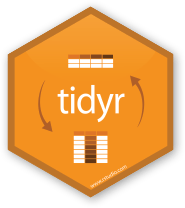
\includegraphics{tidyr.png}

Given a two dimensional data structure, we can think of several ways we
might want to extract data. The first is to extract rows associated with
a certain feature. For example, if we had some basic data from an APFT
test, we may want to extract rows based on GENDER, as seen below.

\begin{figure}[htbp]
\centering
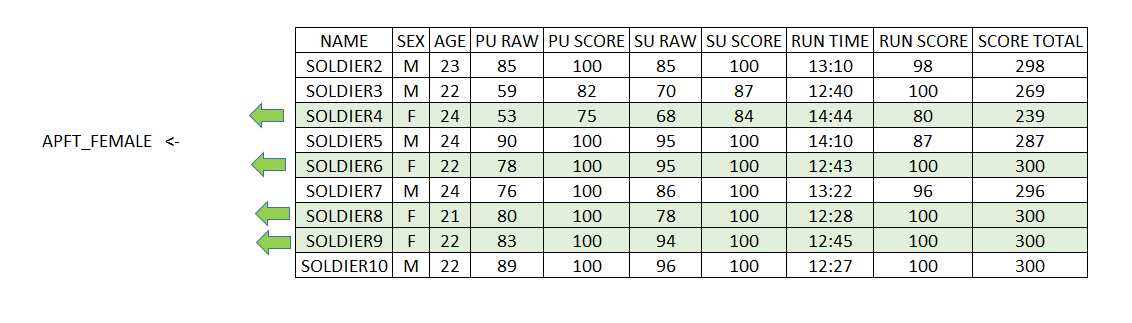
\includegraphics{filterRow.PNG}
\caption{Figure 2: Filtering Rows by Categorical Variable}
\end{figure}

If we were going to conduct this same operation (extract all FEMALE
records) on our \texttt{kor} data frame with the \texttt{dplyr} package,
we would execute the following command:

\begin{Shaded}
\begin{Highlighting}[]
\KeywordTok{library}\NormalTok{(dplyr)}
\NormalTok{kor_female <-}\StringTok{ }\NormalTok{dplyr::}\KeywordTok{filter}\NormalTok{(kor, SEX==}\StringTok{"F"}\NormalTok{)}
\end{Highlighting}
\end{Shaded}

This command should produce a new data frame in your environment that
has has two rows and 25 columns. This new data frame only contains the
two FEMALE casualties represented in the data. To explore this much
smaller data set, we could now table the data frame based on state:

\begin{Shaded}
\begin{Highlighting}[]
\KeywordTok{table}\NormalTok{(kor_female$HOME_STATE)}
\end{Highlighting}
\end{Shaded}

\begin{verbatim}
## 
##          IOWA WEST VIRGINIA 
##             1             1
\end{verbatim}

and find out that one woman is from Iowa, and the other from West
Virginia. If we table based on rank:

\begin{Shaded}
\begin{Highlighting}[]
\KeywordTok{table}\NormalTok{(kor_female$RANK)}
\end{Highlighting}
\end{Shaded}

\begin{verbatim}
## 
## 1STLT 
##     2
\end{verbatim}

we find out that both women were junior officers. If you take a look at
the data further, you will learn that both women were in the Air Force
and died in a non-hostile accident in 1952 on the same day (presumably
the same accident).

Note that we can also filter rows based on a boolean function. For
example, if we wanted to only look at casualties that were over 30 years
old in 1950, we could filter with the following \texttt{dplyr} command:

\begin{Shaded}
\begin{Highlighting}[]
\NormalTok{kor_Over30 <-}\StringTok{ }\KeywordTok{filter}\NormalTok{(kor, BIRTH_YEAR <}\StringTok{ }\DecValTok{1920}\NormalTok{)  ##Filter those older than 30 in 1950}
\end{Highlighting}
\end{Shaded}

When you run this command, you will find that our cleaned data produces
2220 records of casualties that were over 30 in the year 1950. If we
wanted to only select those individuals that were in their 30's in 1950,
we would use the following \texttt{dplyr} command:

\begin{Shaded}
\begin{Highlighting}[]
\NormalTok{kor_30s <-}\StringTok{ }\KeywordTok{filter}\NormalTok{(kor, BIRTH_YEAR <}\StringTok{ }\DecValTok{1920} \NormalTok{&}\StringTok{ }\NormalTok{BIRTH_YEAR >}\StringTok{ }\DecValTok{1910}\NormalTok{)}
\end{Highlighting}
\end{Shaded}

Running this command we find that 1,991 of the casualties were in their
30's in 1950.

Now that we've filtered by row, let's show how to filter by column.
We've already demonstrated above how to do this with the bracket
notation, now we will illustrate how to do this using the \texttt{dplyr}
pacakge. We often find that we've loaded data that has many columns that
we're not interested in. In these cases, it is often helpful to extract
the columns that we're interested in. This will also shrink the size of
our data in memory, and make our code run faster. In the picture below,
we illustrate this with some simple APFT data (in this case we're
extracting the demographic and raw score columns):

\begin{figure}[htbp]
\centering
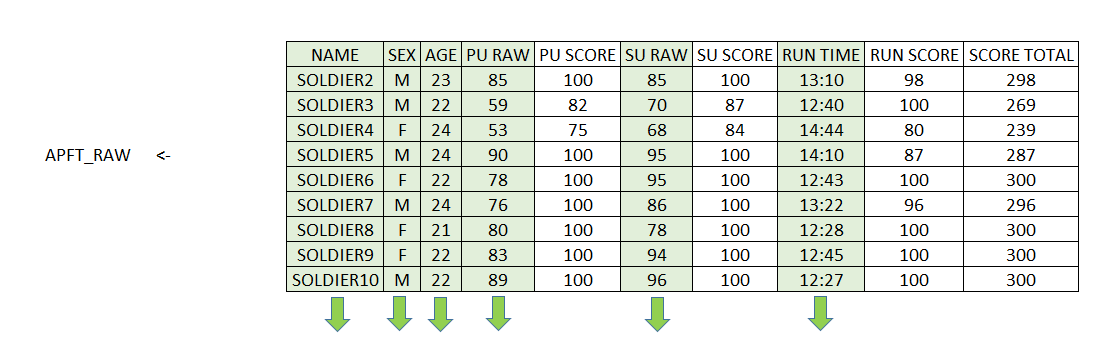
\includegraphics{filterColumn.PNG}
\caption{Figure 3: Filtering Specific Columns (or fields)}
\end{figure}

Let's say we were studying the Korean Casualty data to understand the
time factor of those who died of wounds, and were particulary interested
in the time between \texttt{INCIDENT\_DATE} and \texttt{FATALITY\_DATE}.
Below we'll extract these two columns with the \texttt{dplyr} package:

\begin{Shaded}
\begin{Highlighting}[]
\NormalTok{kor_dates <-}\StringTok{ }\KeywordTok{select}\NormalTok{(kor, }\KeywordTok{one_of}\NormalTok{(}\KeywordTok{c}\NormalTok{(}\StringTok{"INCIDENT_DATE"}\NormalTok{,}\StringTok{"FATALITY_DATE"}\NormalTok{))) }\CommentTok{#Select two columns}
\end{Highlighting}
\end{Shaded}

Now if we look at the structure of this new data frame:

\begin{Shaded}
\begin{Highlighting}[]
\KeywordTok{str}\NormalTok{(kor_dates)}
\end{Highlighting}
\end{Shaded}

\begin{verbatim}
## 'data.frame':    33899 obs. of  2 variables:
##  $ INCIDENT_DATE: chr  "19510412" "19500727" "19510316" "19530122" ...
##  $ FATALITY_DATE: chr  "20010402" "19500727" "19510316" "19530122" ...
\end{verbatim}

We see that we only have two columns, but still have all 33,899 rows.
The code below is beyond the extent of this lesson on filtering (it
contains some code we'll go over in Lesson 5) but is interesting to look
at the difference between incident date and fatality date. In this code
we will load the \texttt{lubridate} package \citep{R-lubridate} (another
package written by Hadley Wickam) and use it to convert these two
columns to date format and calculate the difference between them
(i.e.~the number of days between the incident that the death of the
Service Member).

\begin{Shaded}
\begin{Highlighting}[]
\KeywordTok{library}\NormalTok{(lubridate)}
\NormalTok{days <-}\StringTok{ }\KeywordTok{ymd}\NormalTok{(kor_dates$FATALITY_DATE) -}\StringTok{ }\KeywordTok{ymd}\NormalTok{(kor_dates$INCIDENT_DATE)}
\NormalTok{days[}\DecValTok{1}\NormalTok{:}\DecValTok{100}\NormalTok{]}
\end{Highlighting}
\end{Shaded}

\begin{verbatim}
## Time differences in days
##   [1] 18253     0     0     0     0     0     0     0     0     0 17697
##  [12]     0     0     0 18342    31     0     0     0  1153     0     3
##  [23]     0     0   355     0     0     0     0     0     0     0    53
##  [34]     0     0     0     0     0     0     0     0    NA     0     0
##  [45]    NA   469     0     0    NA     0     0   981     0     0     0
##  [56]     0     0  1131  1155    46     0     0     0     0     0    NA
##  [67]     0    NA     0  1125   959     0   469     0     0     0   969
##  [78]     0     0    31     0  1130     0     0     0 17568     0  1155
##  [89]   120     0   177     0   154     0     0     7     0     0    NA
## [100]     0
\end{verbatim}

Looking at the first few entries makes us wonder. The very first entry
had 18,253 days between the incident and the fatality. In fact, if you
look closer at the dates, you will see that this Service Member had an
incident on 12 April 1951, but wasn't considered a fatality until 2
April 2001. In fact, if we quickly plot a histogram of the difference in
days (you'll learn this command next lesson):

\begin{Shaded}
\begin{Highlighting}[]
\CommentTok{#plot histogram of difference in days}
\KeywordTok{hist}\NormalTok{(}\KeywordTok{as.numeric}\NormalTok{(days), }\DataTypeTok{main=}\StringTok{"Histogram of Difference in Days"}\NormalTok{, }\DataTypeTok{xlab=}\StringTok{"Days"}\NormalTok{)  }
\end{Highlighting}
\end{Shaded}

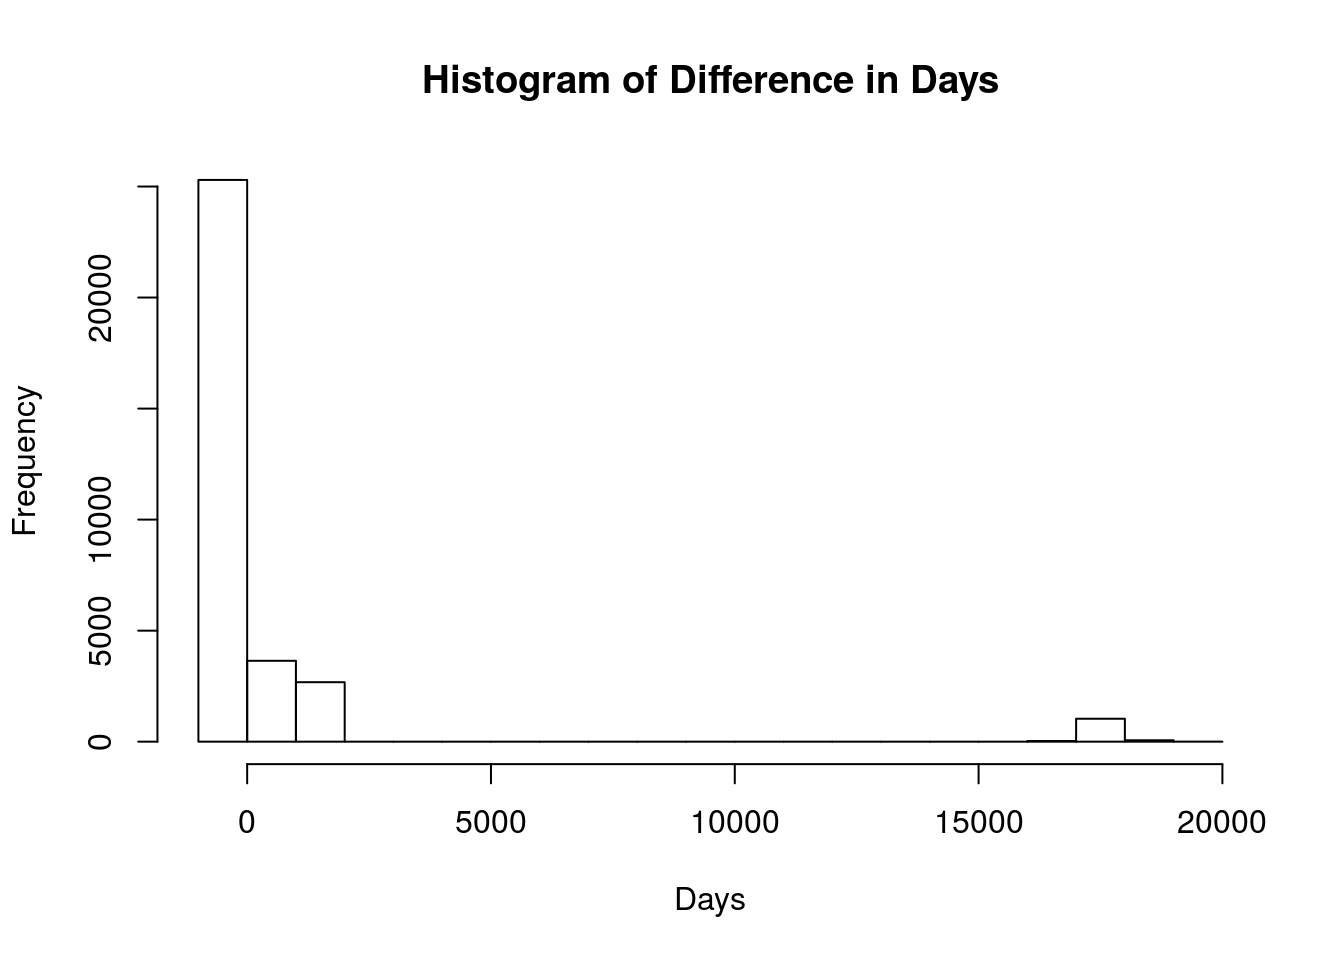
\includegraphics{bookdown-demo_files/figure-latex/unnamed-chunk-56-1.pdf}

Here we see that there's a number of casualties that seem to have a
fatality day around the year 2000. If you look at the original data will
see that the first Service Member in the data (an Air Force Captain) is
listed with an incident year of 1951 and \texttt{FATALITY\_DATE} in
2001. Notice that the FATALITY status is \emph{DECLARED DEAD}. This
officer, as part of a bombing group, must have had an MIA status for
several decades until finally ``declared dead'' in 2001. The ``declared
dead'' date became his fatality date, which means it would be difficult
to evaluate the temporal aspect of wound care with this data.

\section{Using the grep and aggregate
commands}\label{using-the-grep-and-aggregate-commands}

The following video illustrates how to use the grep and aggregate
commands.

\section{Summary}\label{summary}

What we have seen is that R produces a great platform to rapidly
``wrangle'' and explore data.

\section{Homework}\label{homework}

\begin{enumerate}
\def\labelenumi{\arabic{enumi}.}
\tightlist
\item
  Use grep to determine how many casualties had ``infantry'' somewhere
  in their title
\end{enumerate}

\chapter{Basic Visualization}\label{basic-visualization}

The R Programming language has some of the most powerful data
visualization packages available. These packages are continually
expanded upon, with new data visualizations packages being created on a
regular basis. In addition to packages that create your basic
statistical visualization (line plots, bar plots, pie plots, etc) there
are packages that create geospatial visualizations, 3D visualizations,
as well as interactive visualizations.

Lets start by reading in the Korean Conflict data and perform the
primary cleaning functions that we performed last lesson.

\begin{Shaded}
\begin{Highlighting}[]
\NormalTok{kor <-}\StringTok{ }\KeywordTok{read.csv}\NormalTok{(}\StringTok{'KoreanConflict.csv'}\NormalTok{, }\DataTypeTok{as.is=}\OtherTok{TRUE}\NormalTok{)}
\NormalTok{kor$BIRTH_YEAR <-}\StringTok{ }\KeywordTok{as.numeric}\NormalTok{(kor$BIRTH_YEAR)}
\NormalTok{kor <-}\StringTok{ }\NormalTok{kor[!}\KeywordTok{is.na}\NormalTok{(kor$BIRTH_YEAR),]}
\end{Highlighting}
\end{Shaded}

Now that we have the data in memory, we will use some basic
visualizations to explore the data. In this lesson, we will primarily
use visualizations from the ggplot2 package \citep{R-ggplot2}. If you
haven't installed this package yet, run the command
\texttt{install.packages(\textquotesingle{}ggplot2\textquotesingle{})}.

\section{Video on basics of ggplot2}\label{video-on-basics-of-ggplot2}

\section{Basic statistical plots}\label{basic-statistical-plots}

We will start by producing a basic barplot of categorical variables. We
will start by plotting the barplot of \emph{BRANCH} for the Korean
Casualties.

\begin{Shaded}
\begin{Highlighting}[]
\KeywordTok{library}\NormalTok{(ggplot2)}
\KeywordTok{ggplot}\NormalTok{(kor, }\KeywordTok{aes}\NormalTok{(BRANCH)) +}\StringTok{ }\KeywordTok{geom_bar}\NormalTok{()}
\end{Highlighting}
\end{Shaded}

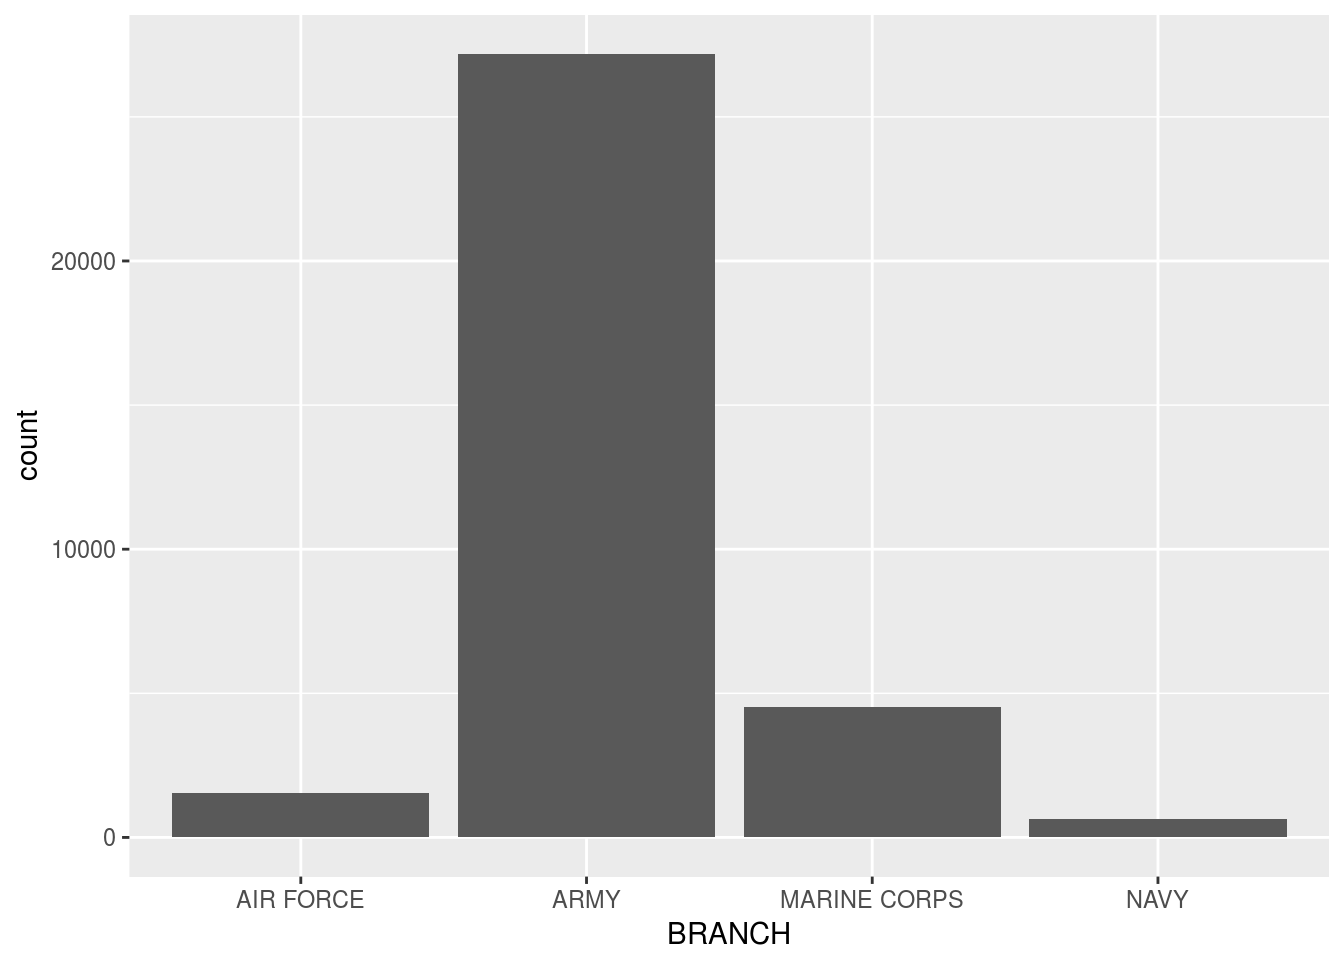
\includegraphics{bookdown-demo_files/figure-latex/unnamed-chunk-58-1.pdf}

If we wanted to improve the color scheme, we could add
\texttt{fill\ =\ BRANCH}.

\begin{Shaded}
\begin{Highlighting}[]
\KeywordTok{ggplot}\NormalTok{(kor, }\KeywordTok{aes}\NormalTok{(BRANCH, }\DataTypeTok{fill =} \NormalTok{BRANCH)) +}\StringTok{ }\KeywordTok{geom_bar}\NormalTok{()}
\end{Highlighting}
\end{Shaded}

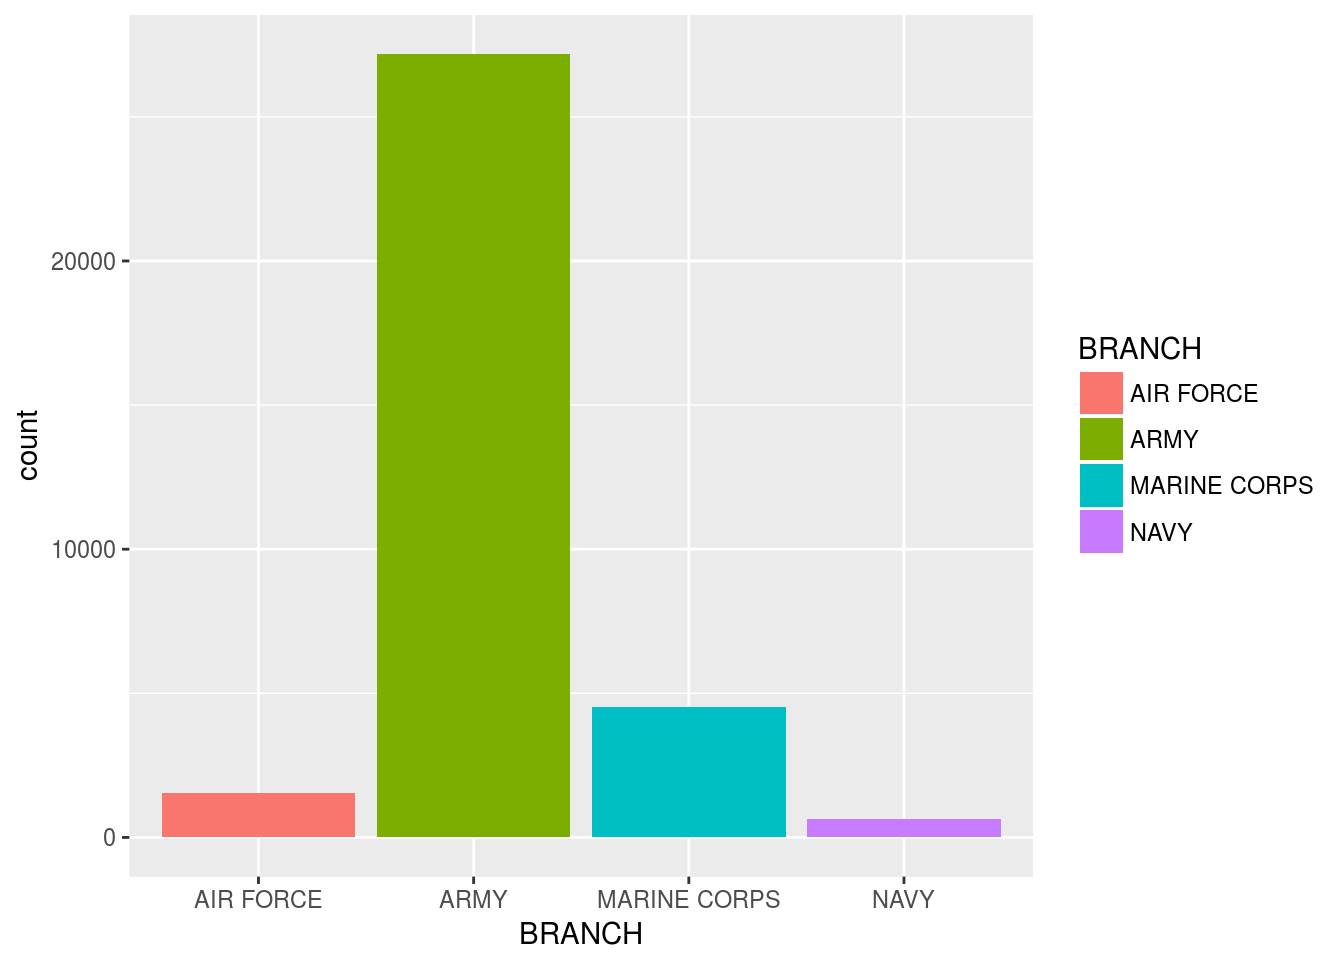
\includegraphics{bookdown-demo_files/figure-latex/unnamed-chunk-59-1.pdf}

Now, let's add a title. Additionally, we will get rid of the legend,
since it the labels are already on the axis.

\begin{Shaded}
\begin{Highlighting}[]
\KeywordTok{ggplot}\NormalTok{(kor, }\KeywordTok{aes}\NormalTok{(BRANCH, }\DataTypeTok{fill =} \NormalTok{BRANCH)) +}\StringTok{ }\KeywordTok{geom_bar}\NormalTok{() +}\StringTok{ }
\StringTok{  }\KeywordTok{ggtitle}\NormalTok{(}\StringTok{"Casualties by Service"}\NormalTok{)+}\StringTok{ }\KeywordTok{theme}\NormalTok{(}\DataTypeTok{legend.position=}\StringTok{"none"}\NormalTok{)}
\end{Highlighting}
\end{Shaded}

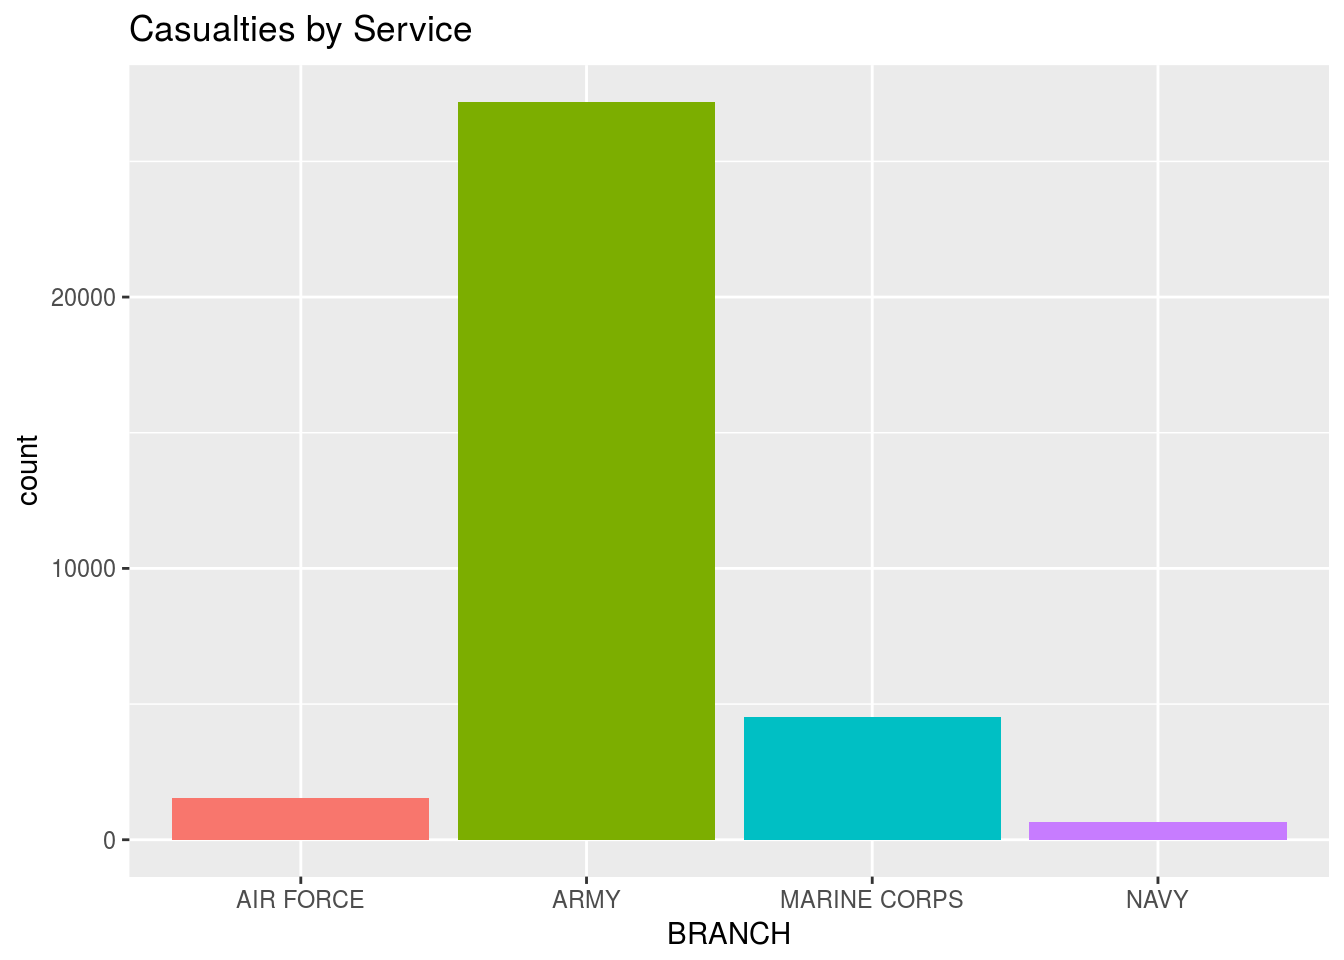
\includegraphics{bookdown-demo_files/figure-latex/unnamed-chunk-60-1.pdf}

What if we wanted to stacked barplot? Say we wanted to see how the
distribution of ETHNICITY in the service BRANCHES. First, let's take a
look at our categories:

\begin{Shaded}
\begin{Highlighting}[]
\KeywordTok{table}\NormalTok{(kor$ETHNICITY_2)}
\end{Highlighting}
\end{Shaded}

\begin{verbatim}
## 
##             AMERICAN INDIAN/ALASKA NATIVE 
##                                       103 
##                                     ASIAN 
##                                       229 
##                 BLACK OR AFRICAN AMERICAN 
##                                      1146 
##                 BLACK OR AFRICAN AMERICAN 
##                                      3022 
##                         HISPANIC ONE RACE 
##                                       566 
## NATIVE HAWAIIAN OR OTHER PACIFIC ISLANDER 
##                                       142 
##                                     WHITE 
##                                     28691
\end{verbatim}

These are rather long names to display on a chart. We will start by
creating shorter names. We can do this in the code below:

\begin{Shaded}
\begin{Highlighting}[]
\NormalTok{kor$ETHNICITY_2[}\KeywordTok{grep}\NormalTok{(}\StringTok{"HAWAIIAN"}\NormalTok{,kor$ETHNICITY_2)] <-}\StringTok{ "HAWAIIAN"}
\end{Highlighting}
\end{Shaded}

Now all we have to do to change in our previous code is to change the
\texttt{fill\ =\ BRANCH} to \texttt{fill\ =\ ETHNICITY\_2}:

\begin{Shaded}
\begin{Highlighting}[]
\KeywordTok{ggplot}\NormalTok{(kor, }\KeywordTok{aes}\NormalTok{(BRANCH, }\DataTypeTok{fill =} \NormalTok{ETHNICITY_2)) +}\StringTok{ }\KeywordTok{geom_bar}\NormalTok{() +}\StringTok{ }
\StringTok{  }\KeywordTok{ggtitle}\NormalTok{(}\StringTok{"Casualties by Service"}\NormalTok{)}
\end{Highlighting}
\end{Shaded}

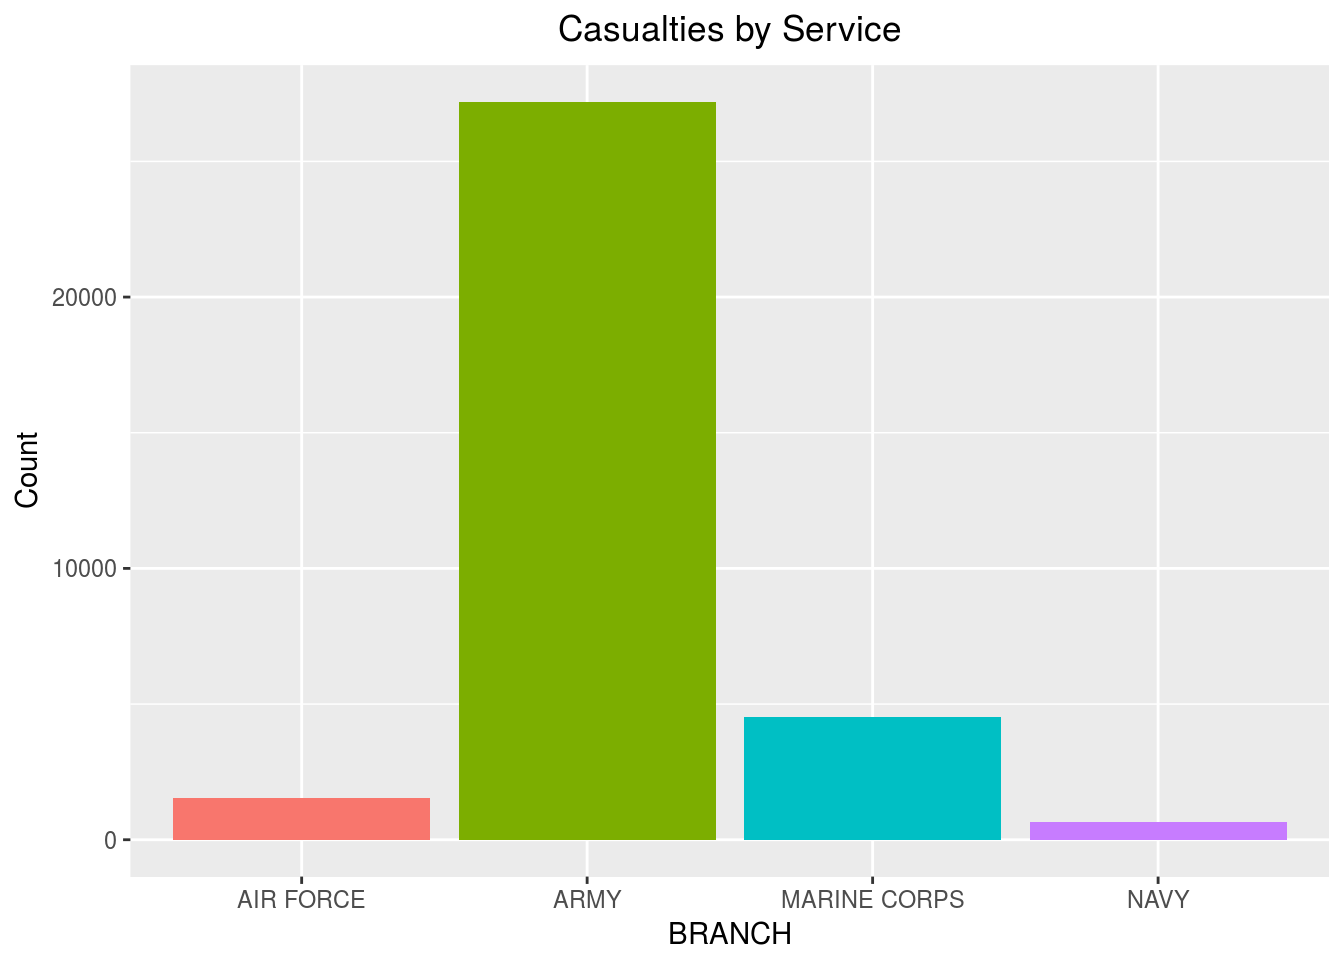
\includegraphics{bookdown-demo_files/figure-latex/unnamed-chunk-63-1.pdf}

Statisticians will generally tell you that you should never use a Pie
Plot (usually a bar plot is recommended because it is easier for a human
eye to distinguish differences in magnitude). That being said, there are
still a few occasional times when a pie plot is necessary. For this
plot, we are going to use a function from the BASE graphics package
(this comes with R and you don't have to load it). The pie plot is very
easy to produce if we wrap the \texttt{pie()} command around the table
function:

\begin{Shaded}
\begin{Highlighting}[]
\KeywordTok{pie}\NormalTok{(}\KeywordTok{table}\NormalTok{(kor$BRANCH), }\DataTypeTok{main =} \StringTok{"Korean War Casualties by Service"}\NormalTok{)}
\end{Highlighting}
\end{Shaded}

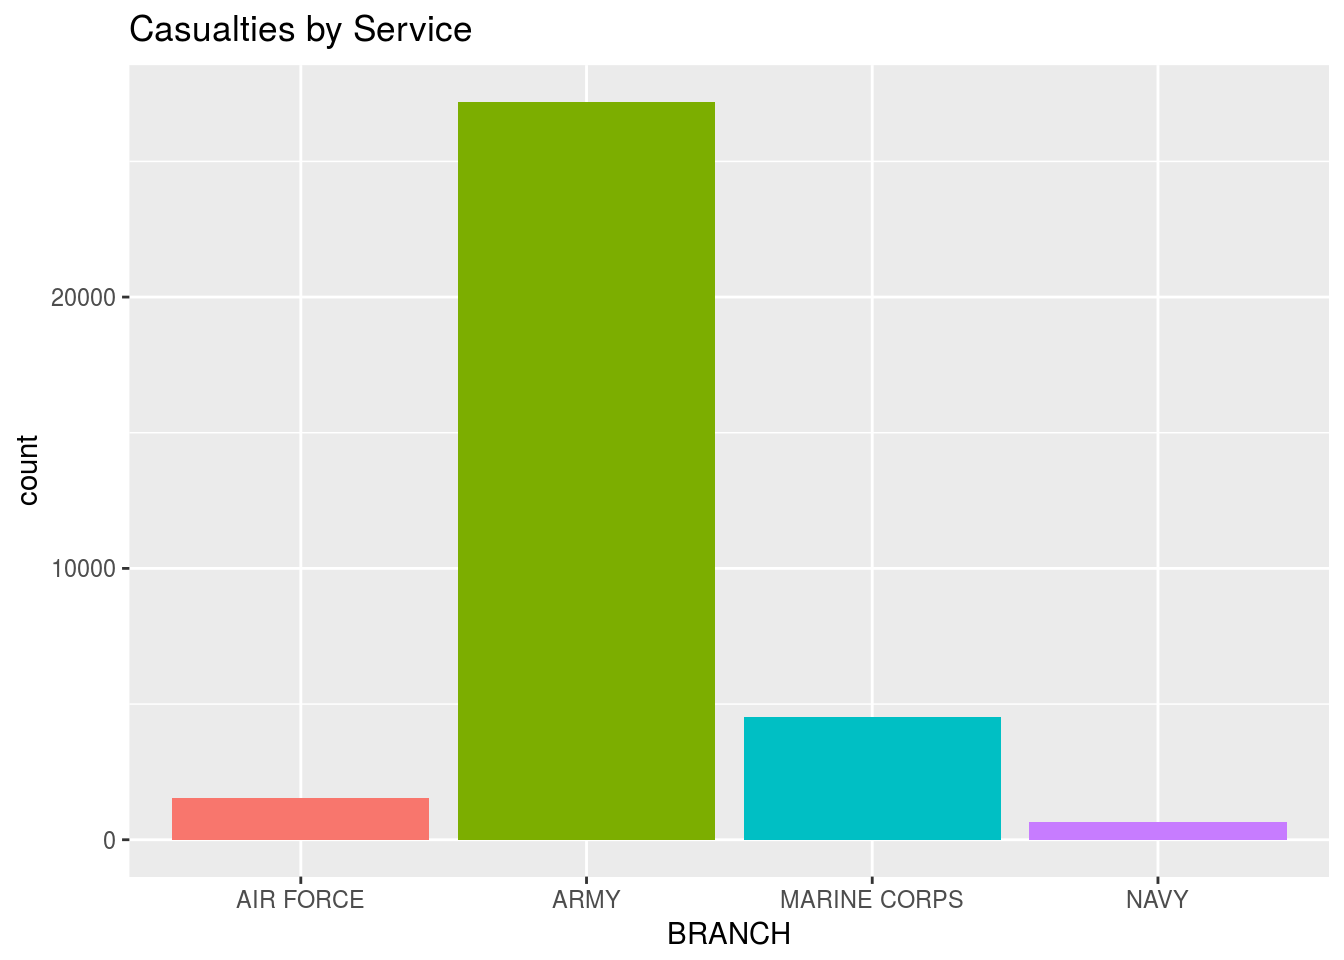
\includegraphics{bookdown-demo_files/figure-latex/unnamed-chunk-64-1.pdf}

\begin{Shaded}
\begin{Highlighting}[]
\NormalTok{kor$FATALITY_YEAR <-}\StringTok{ }\KeywordTok{as.numeric}\NormalTok{(kor$FATALITY_YEAR)}
\end{Highlighting}
\end{Shaded}

\begin{verbatim}
## Warning: NAs introduced by coercion
\end{verbatim}

\begin{Shaded}
\begin{Highlighting}[]
\NormalTok{kor$AGE <-}\StringTok{ }\NormalTok{kor$FATALITY_YEAR -}\StringTok{ }\NormalTok{kor$BIRTH_YEAR}
\end{Highlighting}
\end{Shaded}

\begin{Shaded}
\begin{Highlighting}[]
\KeywordTok{ggplot}\NormalTok{(kor, }\KeywordTok{aes}\NormalTok{(AGE)) +}\StringTok{ }\KeywordTok{geom_histogram}\NormalTok{() +}\StringTok{ }\KeywordTok{ggtitle}\NormalTok{(}\StringTok{'Korean Casualty Age Distribution'}\NormalTok{)}
\end{Highlighting}
\end{Shaded}

\begin{verbatim}
## `stat_bin()` using `bins = 30`. Pick better value with `binwidth`.
\end{verbatim}

\begin{verbatim}
## Warning: Removed 1146 rows containing non-finite values (stat_bin).
\end{verbatim}

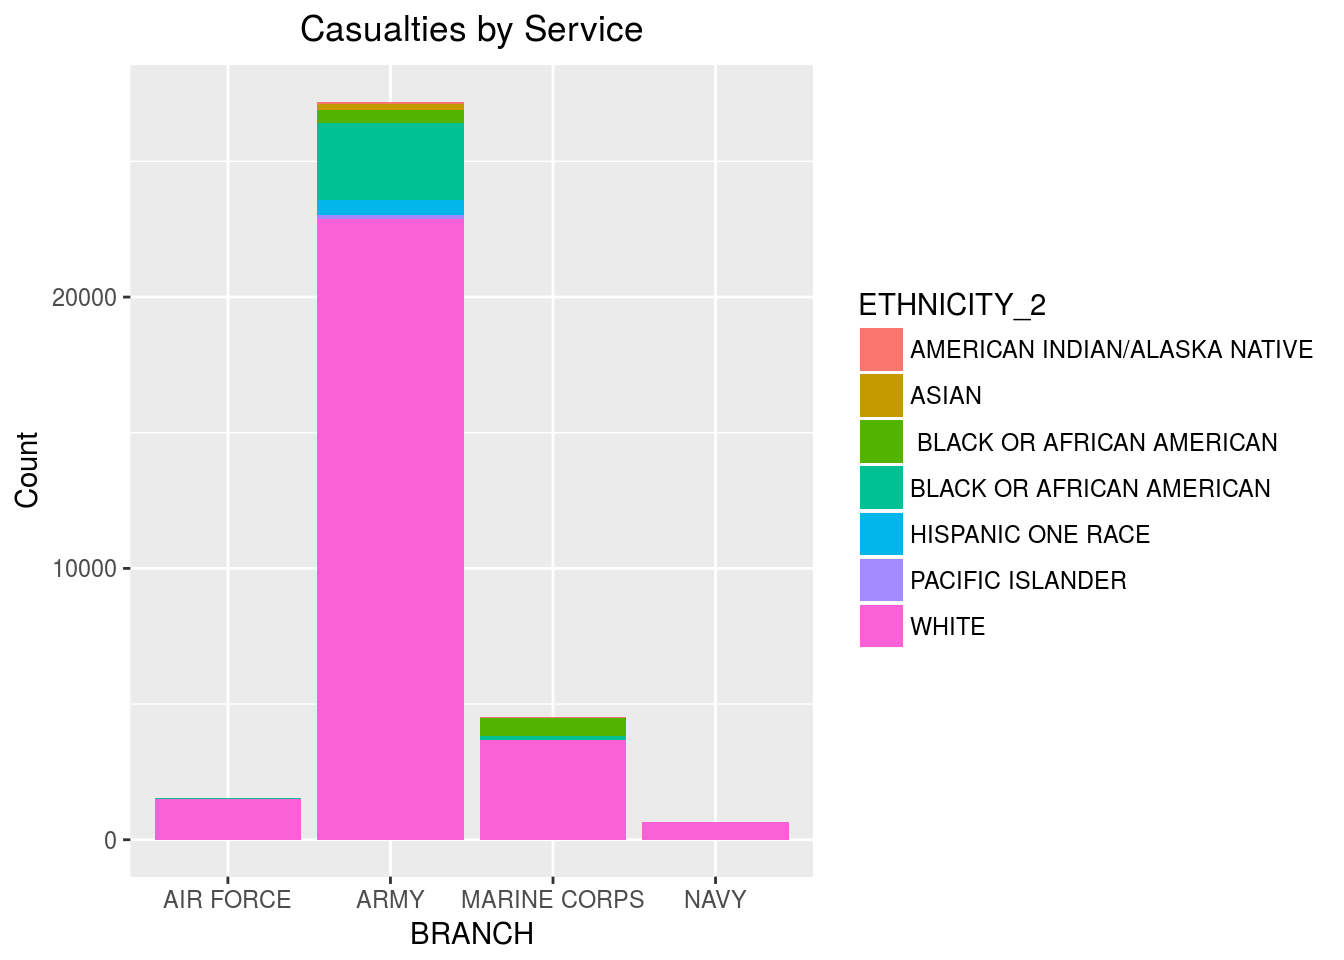
\includegraphics{bookdown-demo_files/figure-latex/unnamed-chunk-66-1.pdf}

\begin{Shaded}
\begin{Highlighting}[]
\NormalTok{##change to horizontal}
\KeywordTok{ggplot}\NormalTok{(kor, }\KeywordTok{aes}\NormalTok{(STATE_CODE)) +}\StringTok{ }\KeywordTok{geom_bar}\NormalTok{() +}\StringTok{ }\KeywordTok{ggtitle}\NormalTok{(}\StringTok{'Korean Casualty Age Distribution'}\NormalTok{) }
\end{Highlighting}
\end{Shaded}

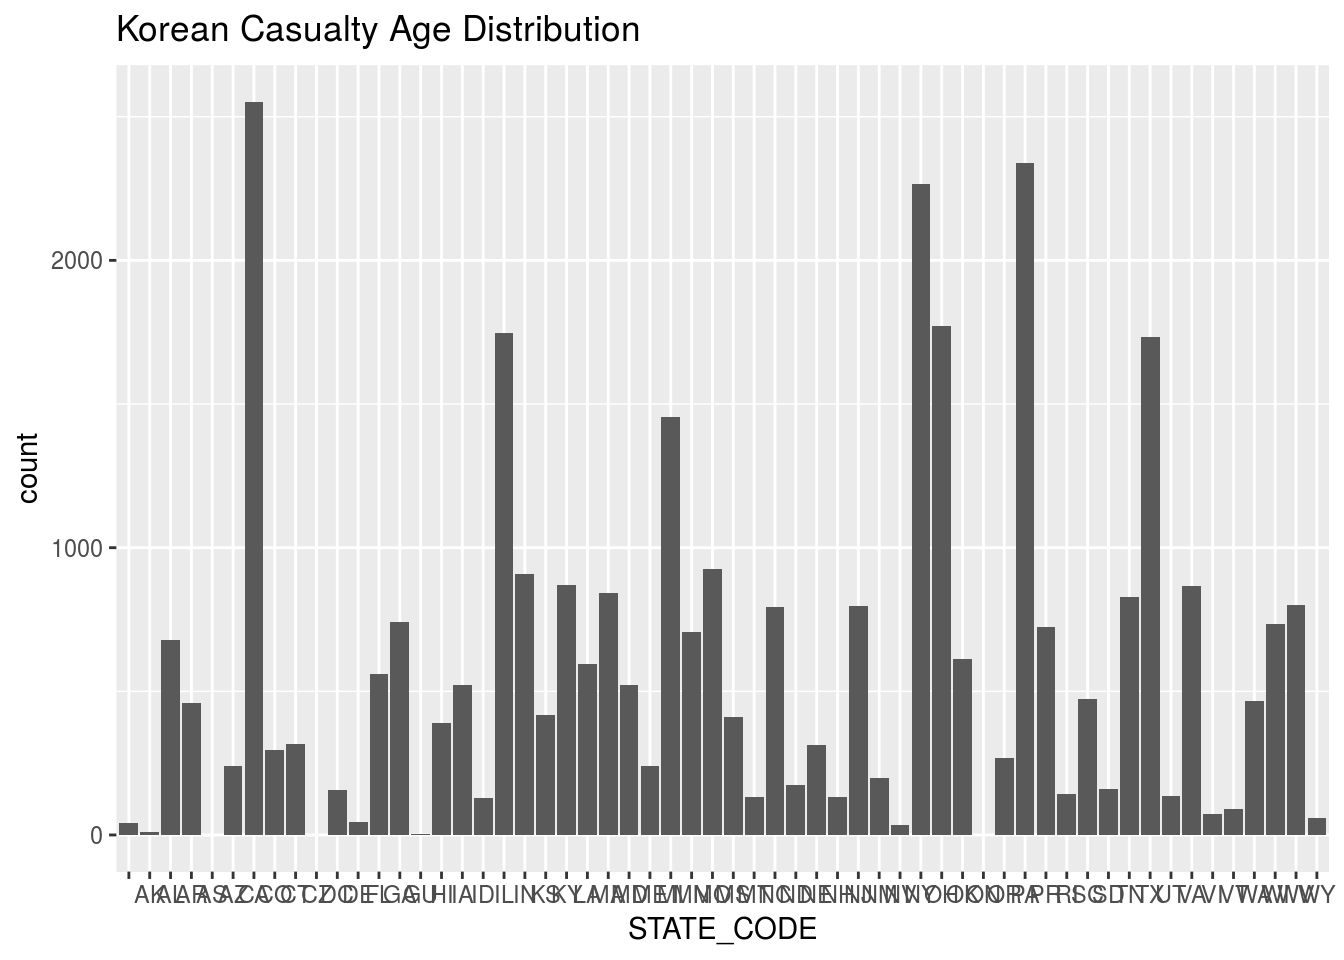
\includegraphics{bookdown-demo_files/figure-latex/unnamed-chunk-67-1.pdf}

\begin{Shaded}
\begin{Highlighting}[]
\NormalTok{oly <-}\StringTok{ }\KeywordTok{read.csv}\NormalTok{(}\StringTok{'summer.csv'}\NormalTok{, }\DataTypeTok{as.is =} \OtherTok{TRUE}\NormalTok{)}
\KeywordTok{str}\NormalTok{(oly)}
\end{Highlighting}
\end{Shaded}

\begin{verbatim}
## 'data.frame':    31165 obs. of  9 variables:
##  $ Year      : int  1896 1896 1896 1896 1896 1896 1896 1896 1896 1896 ...
##  $ City      : chr  "Athens" "Athens" "Athens" "Athens" ...
##  $ Sport     : chr  "Aquatics" "Aquatics" "Aquatics" "Aquatics" ...
##  $ Discipline: chr  "Swimming" "Swimming" "Swimming" "Swimming" ...
##  $ Athlete   : chr  "HAJOS, Alfred" "HERSCHMANN, Otto" "DRIVAS, Dimitrios" "MALOKINIS, Ioannis" ...
##  $ Country   : chr  "HUN" "AUT" "GRE" "GRE" ...
##  $ Gender    : chr  "Men" "Men" "Men" "Men" ...
##  $ Event     : chr  "100M Freestyle" "100M Freestyle" "100M Freestyle For Sailors" "100M Freestyle For Sailors" ...
##  $ Medal     : chr  "Gold" "Silver" "Bronze" "Gold" ...
\end{verbatim}

\begin{Shaded}
\begin{Highlighting}[]
\NormalTok{oly_sum <-}\StringTok{ }\KeywordTok{aggregate}\NormalTok{(Athlete ~}\StringTok{ }\NormalTok{Year +}\StringTok{ }\NormalTok{Gender, }\DataTypeTok{data=}\NormalTok{oly ,length)}
\end{Highlighting}
\end{Shaded}

\begin{Shaded}
\begin{Highlighting}[]
\KeywordTok{ggplot}\NormalTok{(oly_sum, }\KeywordTok{aes}\NormalTok{(Year,Athlete,}\DataTypeTok{group =} \NormalTok{Gender, }\DataTypeTok{color =} \NormalTok{Gender)) +}\StringTok{ }\KeywordTok{geom_line}\NormalTok{() +}\StringTok{ }\KeywordTok{ggtitle}\NormalTok{(}\StringTok{'Summer Olympic Metals by Gender'}\NormalTok{)}
\end{Highlighting}
\end{Shaded}

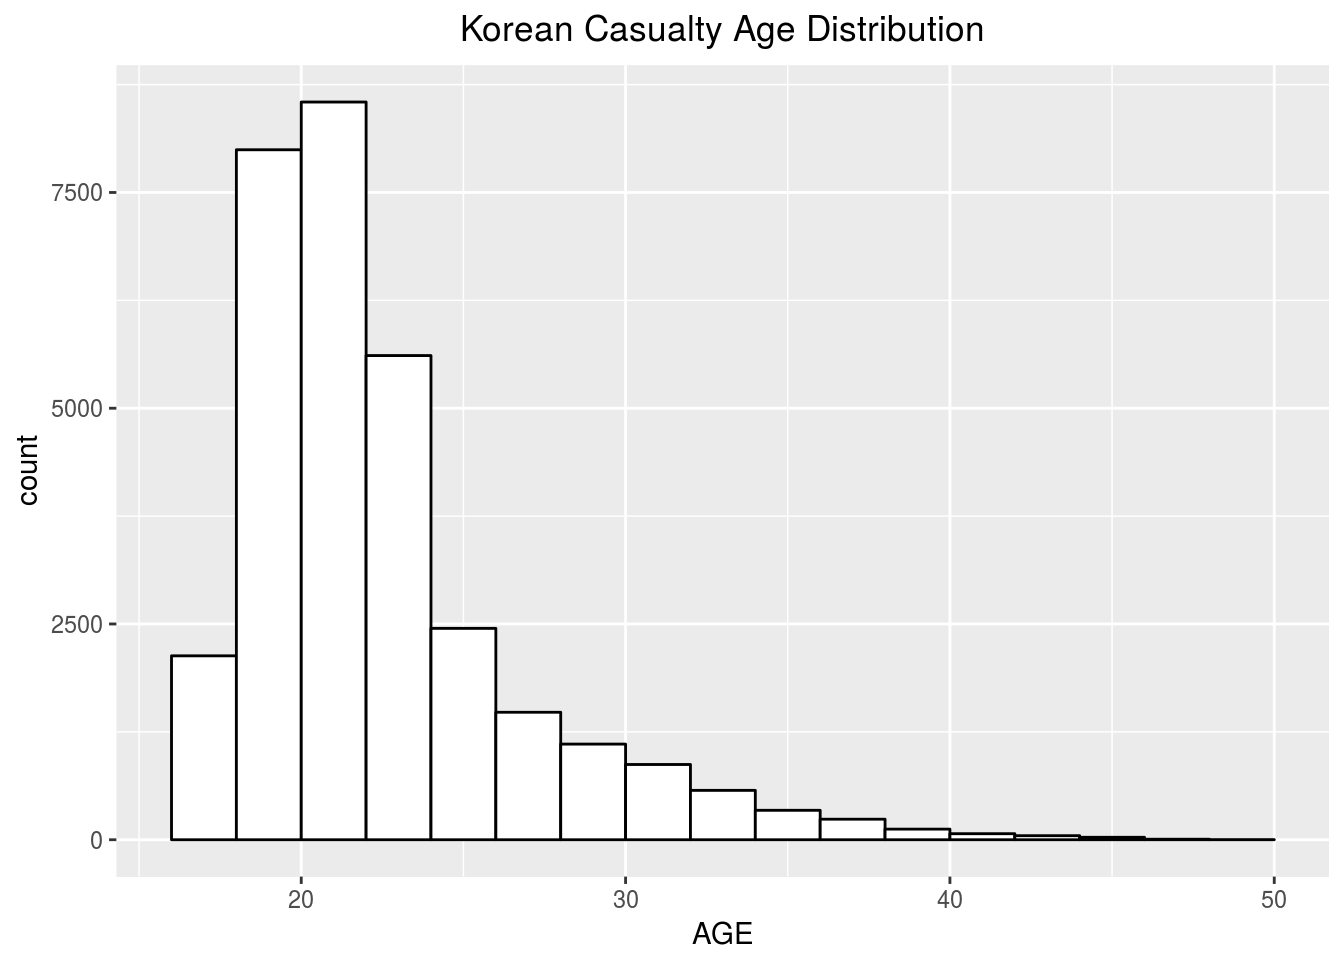
\includegraphics{bookdown-demo_files/figure-latex/unnamed-chunk-70-1.pdf}

\begin{Shaded}
\begin{Highlighting}[]
\KeywordTok{table}\NormalTok{(oly$Country)}
\end{Highlighting}
\end{Shaded}

\begin{verbatim}
## 
##       AFG  AHO  ALG  ANZ  ARG  ARM  AUS  AUT  AZE  BAH  BAR  BDI  BEL  BER 
##    4    2    1   15   29  259   11 1189  146   26   27    1    1  411    1 
##  BLR  BOH  BOT  BRA  BRN  BUL  BWI  CAN  CHI  CHN  CIV  CMR  COL  CRC  CRO 
##  113    7    1  431    1  333    5  649   33  807    1   23   19    4  114 
##  CUB  CYP  CZE  DEN  DJI  DOM  ECU  EGY  ERI  ESP  EST  ETH  EUA  EUN  FIN 
##  410    1   56  507    1    6    2   28    1  442   39   45  260  223  456 
##  FRA  FRG  GAB  GBR  GDR  GEO  GER  GHA  GRE  GRN  GUA  GUY  HAI  HKG  HUN 
## 1396  490    1 1720  825   25 1305   16  148    1    1    1    8    4 1079 
##  INA  IND  IOP  IRI  IRL  IRQ  ISL  ISR  ISV  ITA  JAM  JPN  KAZ  KEN  KGZ 
##   38  184    3   61   30    1   17    7    1 1296  127  788   49   93    3 
##  KOR  KSA  KUW  LAT  LIB  LTU  LUX  MAR  MAS  MDA  MEX  MGL  MKD  MNE  MOZ 
##  529    6    2   20    4   55    2   22    8    6  106   24    1   14    2 
##  MRI  NAM  NED  NGR  NIG  NOR  NZL  PAK  PAN  PAR  PER  PHI  POL  POR  PRK 
##    1    4  851   84    1  554  190  121    3   17   15    9  511   33   58 
##  PUR  QAT  ROU  RSA  RU1  RUS  SCG  SEN  SGP  SIN  SLO  SRB  SRI  SUD  SUI 
##    8    4  640  106   17  768   14    1    4    4   26   31    2    1  380 
##  SUR  SVK  SWE  SYR  TAN  TCH  TGA  THA  TJK  TOG  TPE  TRI  TTO  TUN  TUR 
##    2   34 1044    3    2  329    1   25    3    1   44   20   10   10   86 
##  UAE  UGA  UKR  URS  URU  USA  UZB  VEN  VIE  YUG  ZAM  ZIM  ZZX 
##    1    7  173 2049   76 4585   20   12    2  435    2   23   48
\end{verbatim}

\begin{Shaded}
\begin{Highlighting}[]
\NormalTok{oly$Country[oly$Country==}\StringTok{"URS"}\NormalTok{] <-}\StringTok{ "RUS"}
\end{Highlighting}
\end{Shaded}

\begin{Shaded}
\begin{Highlighting}[]
\KeywordTok{library}\NormalTok{(dplyr)}
\NormalTok{oly_country <-}\StringTok{ }\KeywordTok{aggregate}\NormalTok{(Medal ~}\StringTok{ }\NormalTok{Country +}\StringTok{ }\NormalTok{Year, }\DataTypeTok{data =} \NormalTok{oly, length)}

\NormalTok{countries <-}\StringTok{ }\KeywordTok{c}\NormalTok{(}\StringTok{'USA'}\NormalTok{,}\StringTok{'GBR'}\NormalTok{,}\StringTok{'FRA'}\NormalTok{,}\StringTok{'CHN'}\NormalTok{,}\StringTok{'RUS'}\NormalTok{)}
\NormalTok{oly_country2 <-}\StringTok{ }\KeywordTok{filter}\NormalTok{(oly_country, Country %in%}\StringTok{ }\NormalTok{countries)}
\end{Highlighting}
\end{Shaded}

\begin{Shaded}
\begin{Highlighting}[]
\KeywordTok{ggplot}\NormalTok{(oly_country2, }\KeywordTok{aes}\NormalTok{(Year,Medal,}\DataTypeTok{group =} \NormalTok{Country, }\DataTypeTok{color =} \NormalTok{Country)) +}\StringTok{ }\KeywordTok{geom_line}\NormalTok{() +}\StringTok{ }\KeywordTok{ggtitle}\NormalTok{(}\StringTok{'Summer Olympic Metals by Country'}\NormalTok{)}
\end{Highlighting}
\end{Shaded}

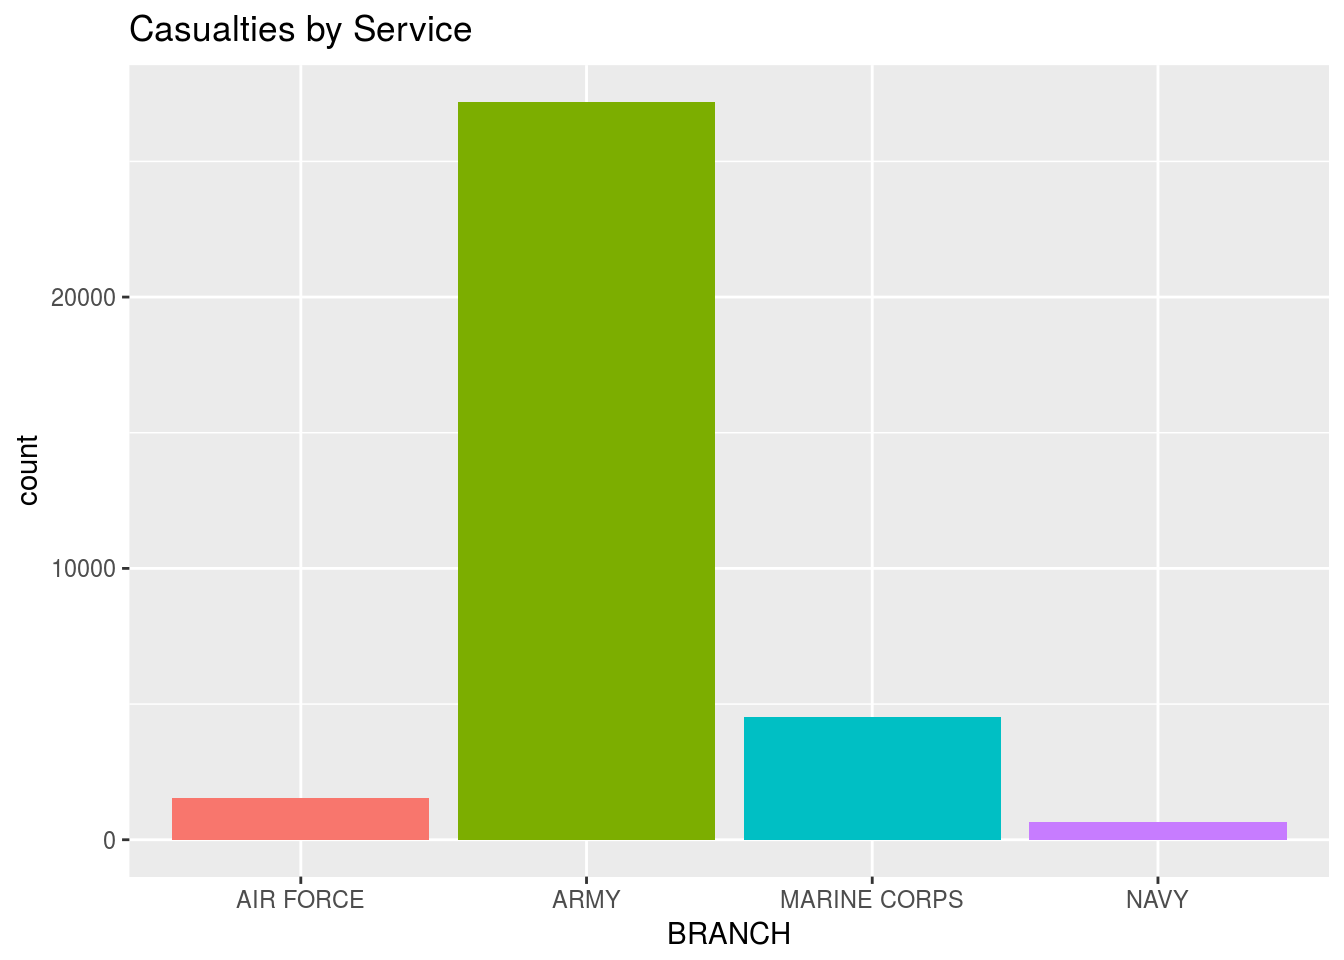
\includegraphics{bookdown-demo_files/figure-latex/unnamed-chunk-74-1.pdf}

\chapter{Introduction to Control
Structures}\label{introduction-to-control-structures}

This lesson will cover the \emph{if-then} statement as well as the
\emph{for} loop and \emph{while} loop. These are two very common control
structures for all computer programming languages, and are used
extensively in the R Programming Language.

\section{If - else Statements}\label{if---else-statements}

The \emph{if-then} statement allows us to automate decision points and
guide the computer through a data flow diagram. The basic syntax is
given below:

\begin{Shaded}
\begin{Highlighting}[]
\NormalTok{if(<condition>) \{}
  \NormalTok{## do something}
\NormalTok{\} else if\{}
  \NormalTok{## do something else}
\NormalTok{\} else \{}
  \NormalTok{## do something completely different}
\NormalTok{\}}
\end{Highlighting}
\end{Shaded}

The else clause is not always necessary, and many times we just need an
if statement:

\begin{Shaded}
\begin{Highlighting}[]
\NormalTok{if(<condition>)}
\end{Highlighting}
\end{Shaded}

The \emph{if-else} statement is most often used in \emph{loops} and
\emph{functions}. We'll illustrate the use of the \emph{if-then}
statement in \emph{loops} below.

\section{Loops}\label{loops}

Loops provide a way to systematically walk down a data structure
(usually a vector, data frame, or list) and accomplish a task. The
\emph{for} loop and the \emph{while} loop will be the primary loops for
this class. The \emph{for} loop is used when we know ahead of time a
finite number of iterations that we need to accomplish.

The \emph{for} loop below iterates over the values 1, 2, 3, 4, and 5 and
prints each of the values.

\begin{Shaded}
\begin{Highlighting}[]
\NormalTok{for(i in }\DecValTok{1}\NormalTok{:}\DecValTok{5}\NormalTok{)\{}
  \KeywordTok{print}\NormalTok{(i)}
\NormalTok{\}}
\end{Highlighting}
\end{Shaded}

\begin{verbatim}
## [1] 1
## [1] 2
## [1] 3
## [1] 4
## [1] 5
\end{verbatim}

Notice that we can also use i to access a value in a vector, a row in a
data frame, or an object in a list.

\begin{Shaded}
\begin{Highlighting}[]
\NormalTok{letters <-}\StringTok{ }\KeywordTok{c}\NormalTok{(}\StringTok{"a"}\NormalTok{, }\StringTok{"b"}\NormalTok{, }\StringTok{"c"}\NormalTok{, }\StringTok{"d"}\NormalTok{, }\StringTok{"e"}\NormalTok{, }\StringTok{"f"}\NormalTok{)}

\NormalTok{for(i in }\DecValTok{1}\NormalTok{:}\DecValTok{4}\NormalTok{)\{}
  \KeywordTok{print}\NormalTok{(letters[i])}
\NormalTok{\}}
\end{Highlighting}
\end{Shaded}

\begin{verbatim}
## [1] "a"
## [1] "b"
## [1] "c"
## [1] "d"
\end{verbatim}

You also don't have to start with 1, or use the letter \emph{i}:

\begin{Shaded}
\begin{Highlighting}[]
\NormalTok{for (year in }\DecValTok{2010}\NormalTok{:}\DecValTok{2015}\NormalTok{)\{}
  \KeywordTok{print}\NormalTok{(}\KeywordTok{paste}\NormalTok{(}\StringTok{"The year is"}\NormalTok{, year))}
\NormalTok{\}}
\end{Highlighting}
\end{Shaded}

\begin{verbatim}
## [1] "The year is 2010"
## [1] "The year is 2011"
## [1] "The year is 2012"
## [1] "The year is 2013"
## [1] "The year is 2014"
## [1] "The year is 2015"
\end{verbatim}

The \emph{next} command is often used to skip an iteration if a certain
condition is met. The code below illustrates how to use the \emph{next}

\begin{Shaded}
\begin{Highlighting}[]
\NormalTok{for(i in }\DecValTok{1}\NormalTok{:}\DecValTok{5}\NormalTok{)\{}
  \NormalTok{if(letters[i]==}\StringTok{"c"}\NormalTok{)\{}
    \NormalTok{next}
  \NormalTok{\}}
  \KeywordTok{print}\NormalTok{(letters[i])}
\NormalTok{\}}
\end{Highlighting}
\end{Shaded}

\begin{verbatim}
## [1] "a"
## [1] "b"
## [1] "d"
## [1] "e"
\end{verbatim}

Loops can also be nested inside of each other. This is useful when
working with multiple dimensions (like matrices) or subsets of subsets
(for example, the outer \emph{for} loop iterates over countries, the
inner \emph{for} loop iterates over each city in a given country. An
example of a nested \emph{for} loop is given below, creating a
multiplication table:

\begin{Shaded}
\begin{Highlighting}[]
\CommentTok{# nested for: multiplication table}
\NormalTok{mymat =}\StringTok{ }\KeywordTok{matrix}\NormalTok{(}\DataTypeTok{nrow=}\DecValTok{10}\NormalTok{, }\DataTypeTok{ncol=}\DecValTok{10}\NormalTok{) }\CommentTok{# create a 30 x 30 matrix (of 30 rows and 30 columns)}

\NormalTok{for(i in }\DecValTok{1}\NormalTok{:}\KeywordTok{nrow}\NormalTok{(mymat)) \{  }\CommentTok{# for each row}
  \NormalTok{for(j in }\DecValTok{1}\NormalTok{:}\KeywordTok{ncol}\NormalTok{(mymat))\{ }\CommentTok{# for each column}
    \NormalTok{mymat[i,j] =}\StringTok{ }\NormalTok{i*j     }\CommentTok{# assign values based on position: product of two indexes}
  \NormalTok{\}}
\NormalTok{\}}

\NormalTok{mymat}
\end{Highlighting}
\end{Shaded}

\begin{verbatim}
##       [,1] [,2] [,3] [,4] [,5] [,6] [,7] [,8] [,9] [,10]
##  [1,]    1    2    3    4    5    6    7    8    9    10
##  [2,]    2    4    6    8   10   12   14   16   18    20
##  [3,]    3    6    9   12   15   18   21   24   27    30
##  [4,]    4    8   12   16   20   24   28   32   36    40
##  [5,]    5   10   15   20   25   30   35   40   45    50
##  [6,]    6   12   18   24   30   36   42   48   54    60
##  [7,]    7   14   21   28   35   42   49   56   63    70
##  [8,]    8   16   24   32   40   48   56   64   72    80
##  [9,]    9   18   27   36   45   54   63   72   81    90
## [10,]   10   20   30   40   50   60   70   80   90   100
\end{verbatim}

The \emph{while} loop is used when we don't know how many iterations we
need to go through, but we know that condition that needs to be met
before we are done.

\begin{Shaded}
\begin{Highlighting}[]
\NormalTok{i <-}\StringTok{ }\DecValTok{5}
\NormalTok{while(i <=}\StringTok{ }\DecValTok{25}\NormalTok{) \{}
  \KeywordTok{print}\NormalTok{(i)}
  \NormalTok{i <-}\StringTok{ }\NormalTok{i +}\StringTok{ }\DecValTok{5}
\NormalTok{\}}
\end{Highlighting}
\end{Shaded}

\begin{verbatim}
## [1] 5
## [1] 10
## [1] 15
## [1] 20
## [1] 25
\end{verbatim}

To finish out this lesson, we'll provide an example below of a little
bit more sophisticated code. This function simulates a round of play in
the boardgame \emph{RISK}. In the boardgame \emph{RISK}, and attacker
begins an assault against a defender, and the win/loss is adjudicated as
both players begin rolling the dice and comparing values. The simulation
below plays through this entire series, declares whether the attacker or
the defender won, and declares the number of armies left on the board
for each player. Instead of doing this once, this code plays through
this 10,000 times, and in the process calculates the probability of the
\emph{attacher} winning. This type of process is known as Monte Carlo
Simulation. Note throughout this function how important \emph{loops} and
\emph{if-else} statements are:

\begin{Shaded}
\begin{Highlighting}[]
\NormalTok{risk<-function(attacker,defender,}\DataTypeTok{n=}\DecValTok{10000}\NormalTok{) \{}
  \NormalTok{results <-}\StringTok{ }\KeywordTok{rep}\NormalTok{(}\OtherTok{NA}\NormalTok{,n)}
\NormalTok{for(j in }\DecValTok{1}\NormalTok{:n)\{}
\NormalTok{while(attacker>}\DecValTok{1} \NormalTok{&}\StringTok{ }\NormalTok{defender>}\DecValTok{0}\NormalTok{) \{}
 \NormalTok{atk.dice<-}\KeywordTok{min}\NormalTok{(attacker}\DecValTok{-1}\NormalTok{,}\DecValTok{3}\NormalTok{)}
 \NormalTok{def.dice<-}\KeywordTok{min}\NormalTok{(defender,}\DecValTok{2}\NormalTok{)}
 \NormalTok{atk.roll<-}\KeywordTok{ceiling}\NormalTok{(}\KeywordTok{runif}\NormalTok{(atk.dice)*}\DecValTok{6}\NormalTok{)}
 \NormalTok{def.roll<-}\KeywordTok{ceiling}\NormalTok{(}\KeywordTok{runif}\NormalTok{(def.dice)*}\DecValTok{6}\NormalTok{)}
 \NormalTok{atk.roll<-atk.roll[}\KeywordTok{order}\NormalTok{(atk.roll,}\DataTypeTok{decreasing=}\NormalTok{T)]}
 \NormalTok{def.roll<-def.roll[}\KeywordTok{order}\NormalTok{(def.roll,}\DataTypeTok{decreasing=}\NormalTok{T)]}
 \NormalTok{comparison<-}\KeywordTok{min}\NormalTok{(atk.dice,def.dice)}
 \NormalTok{for (i in }\DecValTok{1}\NormalTok{:comparison) \{}
  \NormalTok{if (atk.roll[i]>def.roll[i]) defender<-defender}\DecValTok{-1}
  \NormalTok{if (atk.roll[i]<=def.roll[i]) attacker<-attacker}\DecValTok{-1}
 \NormalTok{\}}
\NormalTok{\}}
\NormalTok{if (defender==}\DecValTok{0}\NormalTok{) results[j]<-}\StringTok{"Attacker"}
\NormalTok{if (defender>}\DecValTok{0}\NormalTok{) results[j]<-}\StringTok{"Defender"}
\NormalTok{\}}

\KeywordTok{print}\NormalTok{(}\KeywordTok{paste}\NormalTok{(}\StringTok{"The Probability of the Attacker winning is: "}\NormalTok{,}\KeywordTok{length}\NormalTok{(results[results==}\StringTok{"Attacker"}\NormalTok{])/n))}
\NormalTok{\}}
\end{Highlighting}
\end{Shaded}

Now will illustrate how this function is used:

\begin{Shaded}
\begin{Highlighting}[]
\KeywordTok{risk}\NormalTok{(}\DataTypeTok{attacker=}\DecValTok{12}\NormalTok{,}\DataTypeTok{defender=}\DecValTok{6}\NormalTok{)}
\end{Highlighting}
\end{Shaded}

\begin{verbatim}
## [1] "The Probability of the Attacker winning is:  1"
\end{verbatim}

\chapter{Introduction to Dates in R}\label{introduction-to-dates-in-r}

We often see dates and times in data. Often each record (or row) of data
is connected to at least one date or time. Similar to Microsoft Excel, R
has a special class or format that it uses to work with dates.

\section{Dates with Base R}\label{dates-with-base-r}

We will start by showing a few of the date commands that are built into
the Base R package (later on we will take a look at the \emph{lubridate}
package \citep{R-lubridate}, which has some more user friendly
functions.)

First we will demonstrate a couple commands that will generate the
current date for your system (either your physical computer or your
cloud computer). Below is the system date:

\begin{Shaded}
\begin{Highlighting}[]
\KeywordTok{Sys.Date}\NormalTok{()}
\end{Highlighting}
\end{Shaded}

\begin{verbatim}
## [1] "2017-04-10"
\end{verbatim}

Next we will show the system time down to hours, minutes, and seconds in
Greenwich Mean Time:

\begin{Shaded}
\begin{Highlighting}[]
\KeywordTok{Sys.time}\NormalTok{()}
\end{Highlighting}
\end{Shaded}

\begin{verbatim}
## [1] "2017-04-10 23:36:01 EDT"
\end{verbatim}

Note that if we check the class of either one of these objects, that
neither of these are character objects:

\begin{Shaded}
\begin{Highlighting}[]
\KeywordTok{class}\NormalTok{(}\KeywordTok{Sys.Date}\NormalTok{())}
\end{Highlighting}
\end{Shaded}

\begin{verbatim}
## [1] "Date"
\end{verbatim}

This is a special class called the \emph{Date} class. When you read date
into R, your fields that have dates are normally converted to the
\emph{character} class, not the \emph{date} class. In order to convert
from a \emph{character} class to the \emph{date} class in Base R, use
the code below.

\begin{Shaded}
\begin{Highlighting}[]
\CommentTok{# Create a character vector of random dates}
\NormalTok{myDates <-}\StringTok{ }\KeywordTok{c}\NormalTok{(}\StringTok{"2016-02-07"}\NormalTok{, }\StringTok{"2016-04-02"}\NormalTok{,}\StringTok{"2016-06-28"}\NormalTok{)}

\CommentTok{#Convert character vector to dates vector}
\NormalTok{myDates <-}\StringTok{ }\KeywordTok{as.Date}\NormalTok{(myDates)}

\NormalTok{myDates}
\end{Highlighting}
\end{Shaded}

\begin{verbatim}
## [1] "2016-02-07" "2016-04-02" "2016-06-28"
\end{verbatim}

Now we'll check to make sure we've converted it to the proper class of
data:

\begin{Shaded}
\begin{Highlighting}[]
\KeywordTok{class}\NormalTok{(myDates)}
\end{Highlighting}
\end{Shaded}

\begin{verbatim}
## [1] "Date"
\end{verbatim}

Now that this is a date object, we can conduct mathematical operations
that we could not conduct with a character vector, like subtracting 5
days from all dates:

\begin{Shaded}
\begin{Highlighting}[]
\NormalTok{myDates -}\StringTok{ }\DecValTok{5}
\end{Highlighting}
\end{Shaded}

\begin{verbatim}
## [1] "2016-02-02" "2016-03-28" "2016-06-23"
\end{verbatim}

or checking the difference between dates:

\begin{Shaded}
\begin{Highlighting}[]
\KeywordTok{Sys.Date}\NormalTok{() -}\StringTok{ }\NormalTok{myDates[}\DecValTok{1}\NormalTok{]}
\end{Highlighting}
\end{Shaded}

\begin{verbatim}
## Time difference of 428 days
\end{verbatim}

The date formatting code above will only work as described above if my
input dates are formated exactly as shown, with four-digit years,
two-digit months and days, and hyphens in between. In order to convert
dates in a different format, you will use the format parameter and
describe you unique date format as seen below:

\begin{Shaded}
\begin{Highlighting}[]
\CommentTok{# Create a character vector of random dates}
\NormalTok{myDates <-}\StringTok{ }\KeywordTok{c}\NormalTok{(}\StringTok{"02/07/2016"}\NormalTok{, }\StringTok{"04/02/2016"}\NormalTok{,}\StringTok{"06/28/2016"}\NormalTok{)}

\CommentTok{#Convert character vector to dates vector}
\NormalTok{myDates <-}\StringTok{ }\KeywordTok{as.Date}\NormalTok{(myDates, }\DataTypeTok{format =} \StringTok{"%m/%d/%Y"}\NormalTok{)}

\NormalTok{myDates}
\end{Highlighting}
\end{Shaded}

\begin{verbatim}
## [1] "2016-02-07" "2016-04-02" "2016-06-28"
\end{verbatim}

Below is a table of all the most common date components and their
abbreviation.

\begin{longtable}[]{@{}ll@{}}
\toprule
\begin{minipage}[b]{0.34\columnwidth}\raggedright\strut
Conversion Specification\strut
\end{minipage} & \begin{minipage}[b]{0.48\columnwidth}\raggedright\strut
Definition\strut
\end{minipage}\tabularnewline
\midrule
\endhead
\begin{minipage}[t]{0.34\columnwidth}\raggedright\strut
\%a\strut
\end{minipage} & \begin{minipage}[t]{0.48\columnwidth}\raggedright\strut
Abbreviated weekday\strut
\end{minipage}\tabularnewline
\begin{minipage}[t]{0.34\columnwidth}\raggedright\strut
\%A\strut
\end{minipage} & \begin{minipage}[t]{0.48\columnwidth}\raggedright\strut
Full weekday\strut
\end{minipage}\tabularnewline
\begin{minipage}[t]{0.34\columnwidth}\raggedright\strut
\%b\strut
\end{minipage} & \begin{minipage}[t]{0.48\columnwidth}\raggedright\strut
Abbreviated month\strut
\end{minipage}\tabularnewline
\begin{minipage}[t]{0.34\columnwidth}\raggedright\strut
\%B\strut
\end{minipage} & \begin{minipage}[t]{0.48\columnwidth}\raggedright\strut
Full month\strut
\end{minipage}\tabularnewline
\begin{minipage}[t]{0.34\columnwidth}\raggedright\strut
\%d\strut
\end{minipage} & \begin{minipage}[t]{0.48\columnwidth}\raggedright\strut
Day of the month as decimal number (01--31).\strut
\end{minipage}\tabularnewline
\begin{minipage}[t]{0.34\columnwidth}\raggedright\strut
\%H\strut
\end{minipage} & \begin{minipage}[t]{0.48\columnwidth}\raggedright\strut
Hours as decimal number (00--23)\strut
\end{minipage}\tabularnewline
\begin{minipage}[t]{0.34\columnwidth}\raggedright\strut
\%I\strut
\end{minipage} & \begin{minipage}[t]{0.48\columnwidth}\raggedright\strut
Hours as decimal number (01--12)\strut
\end{minipage}\tabularnewline
\begin{minipage}[t]{0.34\columnwidth}\raggedright\strut
\%m\strut
\end{minipage} & \begin{minipage}[t]{0.48\columnwidth}\raggedright\strut
Month as decimal number (01--12)\strut
\end{minipage}\tabularnewline
\begin{minipage}[t]{0.34\columnwidth}\raggedright\strut
\%M\strut
\end{minipage} & \begin{minipage}[t]{0.48\columnwidth}\raggedright\strut
Minute as decimal number (00--59)\strut
\end{minipage}\tabularnewline
\begin{minipage}[t]{0.34\columnwidth}\raggedright\strut
\%p\strut
\end{minipage} & \begin{minipage}[t]{0.48\columnwidth}\raggedright\strut
AM/PM indicator in the locale. Used in conjunction with \%I and not with
\%H\strut
\end{minipage}\tabularnewline
\begin{minipage}[t]{0.34\columnwidth}\raggedright\strut
\%S\strut
\end{minipage} & \begin{minipage}[t]{0.48\columnwidth}\raggedright\strut
Second as integer (00--61), allowing for up to two leap-seconds\strut
\end{minipage}\tabularnewline
\begin{minipage}[t]{0.34\columnwidth}\raggedright\strut
\%w\strut
\end{minipage} & \begin{minipage}[t]{0.48\columnwidth}\raggedright\strut
Weekday as decimal number (0--6, Sunday is 0).\strut
\end{minipage}\tabularnewline
\begin{minipage}[t]{0.34\columnwidth}\raggedright\strut
\%y\strut
\end{minipage} & \begin{minipage}[t]{0.48\columnwidth}\raggedright\strut
Year with two digits (87)\strut
\end{minipage}\tabularnewline
\begin{minipage}[t]{0.34\columnwidth}\raggedright\strut
\%Y\strut
\end{minipage} & \begin{minipage}[t]{0.48\columnwidth}\raggedright\strut
Year with century (1987)\strut
\end{minipage}\tabularnewline
\begin{minipage}[t]{0.34\columnwidth}\raggedright\strut
\%Z\strut
\end{minipage} & \begin{minipage}[t]{0.48\columnwidth}\raggedright\strut
Time zone abbreviation as a character string (empty if not
available)\strut
\end{minipage}\tabularnewline
\bottomrule
\end{longtable}

\section{Dates with the Lubridate
Package}\label{dates-with-the-lubridate-package}

The \emph{lubridate} package was developed to make date conversions
faster and simpler. This package contains a few basic commands that will
convert all of the most common date formats without the user having to
specify their unique data format.

The basic \emph{lubridate} date conversions are \texttt{ymd}
(year-month-day), \texttt{mdy} (month-day-year), and \texttt{dmy}
(day-month-year).

We've illustrated how to use these functions below:

\begin{Shaded}
\begin{Highlighting}[]
\KeywordTok{library}\NormalTok{(lubridate)}
\KeywordTok{ymd}\NormalTok{(}\StringTok{"2016-02-07"}\NormalTok{, }\StringTok{"2016-04-02"}\NormalTok{,}\StringTok{"2016-06-28"}\NormalTok{)}
\end{Highlighting}
\end{Shaded}

\begin{verbatim}
## [1] "2016-02-07" "2016-04-02" "2016-06-28"
\end{verbatim}

Now we'll use \texttt{mdy} to convert in a different format.

\begin{Shaded}
\begin{Highlighting}[]
\KeywordTok{mdy}\NormalTok{(}\StringTok{"02/07/2016"}\NormalTok{, }\StringTok{"04/02/2016"}\NormalTok{,}\StringTok{"06/28/2016"}\NormalTok{)}
\end{Highlighting}
\end{Shaded}

\begin{verbatim}
## [1] "2016-02-07" "2016-04-02" "2016-06-28"
\end{verbatim}

To show the flexibility of this code, we'll do a final example with
\texttt{dmy} used on a different format data:

\begin{Shaded}
\begin{Highlighting}[]
\KeywordTok{dmy}\NormalTok{(}\StringTok{"1jan16"}\NormalTok{, }\StringTok{"1nov15"}\NormalTok{,}\StringTok{"15mar17"}\NormalTok{)}
\end{Highlighting}
\end{Shaded}

\begin{verbatim}
## [1] "2016-01-01" "2015-11-01" "2017-03-15"
\end{verbatim}

The \emph{lubridate} commands can be expanded to include
hour-minute-seconds as well

\begin{Shaded}
\begin{Highlighting}[]
\KeywordTok{ymd_hms}\NormalTok{(}\StringTok{"2016-10-10 17:46:52"}\NormalTok{, }\StringTok{"2016-11-14 12:04:05"}\NormalTok{, }\StringTok{"2016-10-22 22:44:58"}\NormalTok{)}
\end{Highlighting}
\end{Shaded}

\begin{verbatim}
## [1] "2016-10-10 17:46:52 UTC" "2016-11-14 12:04:05 UTC"
## [3] "2016-10-22 22:44:58 UTC"
\end{verbatim}

If you have times in different time zones, you can add a time zone
parameter:

\begin{Shaded}
\begin{Highlighting}[]
\KeywordTok{ymd_hms}\NormalTok{(}\StringTok{"2016-10-10 17:46:52"}\NormalTok{, }\DataTypeTok{tz=}\StringTok{"Pacific/Aukland"}\NormalTok{)}
\end{Highlighting}
\end{Shaded}

\begin{verbatim}
## [1] "2016-10-10 17:46:52 Pacific"
\end{verbatim}

Note: UTC and GMT are Greenwich Mean Time (also known as ``Zulu'' time).

\section{POSIXct and POSIXlt}\label{posixct-and-posixlt}

To fully understand how dates work in R, you will need study and
understand the POSIXct and POSIXlt classes. You can learn more about
these by typing \texttt{?POSIXct} or \texttt{?POSIXlt} respectively.

\bibliography{packages.bib,book.bib}


\end{document}
